\documentclass[
    %draft, % Mit % kommentieren, um Bilder sichtbar zu machen und Links zu aktivieren
    pdftex,
    a4paper,
    oneside,
    parskip,
    numbers=noenddot,
    listof=totoc,
    bibliography=totoc,
    hyperfootnotes=false
]{scrreprt}
\setuptoc{toc}{totoc}

\newcommand{\thesistitle}{Untersuchung der allgemeinen Anwendbarkeit von Fluxkondensatoren}
\newcommand{\thesistype}{M A S T E R A R B E I T}
\newcommand{\thesistypedesc}{im Fachbereich Elektrotechnik/Informatik \\
    der Universität Kassel}
\newcommand{\thesisauthorname}{Max Mustermann}
\newcommand{\thesisauthorhomestreet}{Beispielstr. 42}
\newcommand{\thesisauthorhometown}{34121 Kassel}
\newcommand{\thesisauthormatrikelnumber}{35123456}
\newcommand{\thesisauthoremail}{max.mustermann@uni-kassel.de}
\newcommand{\thesisdepartment}{Fachgebiet Software Engineering}
\newcommand{\thesisfirstreviewer}{Prof.\ Dr.\ Albert Zündorf}
\newcommand{\thesissecondreviewer}{Prof.\ Dr.\ Emmett Brown}
\newcommand{\thesissupervisor}{Christian Coupé,\ M.Sc.}
\newcommand{\thesisdate}{\today}

% Select input encodung, usually utf8 is the best choice, on windows, \usepackage[latin1]{inputenc} maybe required
\usepackage[utf8]{inputenc}
\usepackage[T1]{fontenc}
\usepackage[ngerman]{babel}
\usepackage{csquotes}
\usepackage{xcolor}

\MakeOuterQuote{"} % Damit ist es möglich, " " zu verwenden ohne Umlaut zu erzeugen
\defaulthyphenchar=127 % Dadurch werden auch Wörter mit Bindestrich getrennt, die schon Bindestriche enthalten.

% geometry
\usepackage[bindingoffset=1cm, left=2.5cm, right=2.5cm, top=2.5cm, bottom=2.5cm]{geometry}

% Headline
\usepackage{fancyhdr}
\pagestyle{fancy}
\renewcommand{\chaptermark}[1]{\markboth{\thechapter\ #1}{}}
\lhead{\leftmark} \rhead{\thepage}
\cfoot{}
\fancypagestyle{plain}{}

\RedeclareSectionCommand[beforeskip=1.5cm,afterskip=1cm]{chapter}

% Colors
\usepackage{color}
\usepackage{colortbl}

% Tables
\usepackage{tabularx}
\usepackage{multirow}
\setlength{\tabcolsep}{4pt}

% Drawing graphs etc.
\usepackage{pgf}
\usepackage{tikz}
\usetikzlibrary{arrows,automata}

% Footnotes
\usepackage{footmisc}

\usepackage{xspace}
\newcommand{\sic}{[\acs{sic}]\xspace}

% math
\usepackage{amsmath}
\usepackage{siunitx}

% lists
\usepackage{paralist}

% Figures
\usepackage{graphicx, wrapfig}
\usepackage{svg}

% Hyperlinks
\usepackage[hyphens]{url}
\usepackage{hyperref}
\hypersetup{colorlinks, citecolor=black, linkcolor=black, urlcolor=black}

% Minted
\usepackage[chapter]{minted}
%\usemintedstyle{xcode}
\setminted{frame=single,tabsize=2,linenos,autogobble}

\newmintinline[code]{text}{breaklines}

\newminted[mdcodeblock]{md}{autogobble,frame=none,linenos=false,breaklines}

% list of abbreviations
\usepackage[printonlyused]{acronym}

% Set line pitch
\usepackage{setspace}
\onehalfspacing              % anderthalbzeilig (oder auch \doublespace)

%fancyBox
%\usepackage{fancybox}

% Layout corrections (Schusterjungen)
\clubpenalty = 10000
% Layout corrections (Hurenkinder)
\widowpenalty = 10000
\displaywidowpenalty = 10000

% Figures
\usepackage{caption}
\usepackage[hypcap=true,labelformat=simple]{subcaption}
\renewcommand{\thesubfigure}{(\alph{subfigure})}

% Tables
\usepackage{booktabs}

% Frequently used column types
\newcolumntype{C}[1]{>{\centering\arraybackslash}p{#1}} % centering column type with fixed width
\newcolumntype{R}[1]{>{\raggedleft\arraybackslash}p{#1}} % right aligned column type with fixed width
\newcolumntype{L}[1]{>{\raggedright\arraybackslash}p{#1}} % left aligned column type with fixed width

% Shortcuts for referencing floats:
\newcommand{\fig}[1]{\figurename~\ref{#1}} %shortcut for a figure reference
\newcommand{\tab}[1]{Table~\ref{#1}} %shortcut for a table reference
\newcommand{\eq}[1]{(\ref{#1})} %shortcut for an equation reference
\newcommand{\lst}[1]{Listing~\ref{#1}} %shortcut for a listing reference
\newcommand{\sect}[1]{Section~\ref{#1}} %shortcut for a Section reference
\newcommand{\br}[0]{\hspace{0cm}\\}


\begin{document}

    \pagenumbering{roman}

    \begin{titlepage}
	%select font without serifs
	\sffamily

	% Logo
	\begin{tabularx}{\textwidth}{@{}l@{}>{\raggedleft\arraybackslash}X@{}r@{}}
		\multirow{2}{*}{
\includegraphics[width=6.8cm]{images/Logo_UniKassel}} &
		\raisebox{-1mm}{\small{Fachbereich Elektrotechnik/Informatik}} \\
		&\raisebox{-1mm}{\small{\thesisdepartment}} &
	\end{tabularx}

	\vspace{2.5cm}

	\begin{center}
		% Title and subtitle
		\huge{\thesistitle}

		\vspace{3cm}

		\renewcommand{\baselinestretch}{1.3}
		\Large{\thesistype}

		\large
		\thesistypedesc
	\end{center}

	\vspace{1.5cm}
	\renewcommand{\baselinestretch}{1}
	\begin{table}[htpb]
		\centering
		\begin{tabular}{ll}
			\\
			Eingereicht von: & \thesisauthorname \\
			Anschrift: & \thesisauthorhomestreet \\
			& \thesisauthorhometown \\
			\\
			Matrikelnummer: & \thesisauthormatrikelnumber \\
			E-Mail: & \thesisauthoremail \\
			\\
			Vorgelegt im: & \thesisdepartment \\
			\\
			Erstprüfer: & \thesisfirstreviewer \\
			Zweitprüferin: & \thesissecondreviewer \\
			\\
			Betreuer: & \thesissupervisor \\
			\\
			Eingereicht am: & \thesisdate \\
		\end{tabular}
	\end{table}

	% font with serifs
	\rmfamily
\end{titlepage}

    \setcounter{page}{0}
\chapter*{Eidesstattliche Erklärung}

Hiermit erkläre ich, dass ich die vorliegende Arbeit selbstständig und nur mit den nach der Prüfungsordnung der Universität Kassel zulässigen Hilfsmitteln angefertigt habe.
Die verwendete Literatur ist im Literaturverzeichnis angegeben.
Wörtlich oder sinngemäß übernommene Inhalte habe ich als solche kenntlich gemacht.

\vspace{1cm}

Kassel, \thesisdate

\begin{flushright}
  \underline{\hspace{7cm}} \\
  \thesisauthorname

  % \underline{\hspace{7cm}} \\
  % Weitere Autoren von Dokumentationen...
\end{flushright}

    \chapter*{Zusammenfassung}

% Inhaltsverzeichnis und Kopfzeile
\addcontentsline{toc}{chapter}{Zusammenfassung}
\markboth{Zusammenfassung}{Zusammenfassung}

In dieser Arbeit werden Speicher- und Ladesysteme von Videospielen betrachtet. Diese Systeme sollen beim Start eines Spieles den Spielstand und während der Spielphase noch weitere benötigten Daten des Spielstandes laden und stets den aktuellen Stand absichern können. Dies sollte möglichst effizient passieren, damit die Systeme die Erfahrung für Spieler nicht stören und im Hintergrund der Anwendung laufen können. Dafür werden verschiedene Methoden des Speicherns und Ladens der Spielobjekte vorgestellt und mittels eines Testszenario und Laufzeitmessungen verglichen. Auf dem Testszenario werden verschiedene Basisfunktionen eines Speicher- und Ladesystems getestet, damit die Stärken und Schwachstellen von jeder Strategie bestimmt werden können. Außerdem wird betrachtet, ob in den populären modernen Game Engines Funktionen eingebaut sind oder Techniken verwendet werden, die das Aufbauen eines Speicher- und Ladesystems erleichtern oder größtenteils übernehmen. Des Weiteren wird untersucht, welche Strategien in der Spieleindustrie verwendet werden. Dazu werden verschiedene populäre Videospiele und deren Strategien des Speicherns und Ladens eines Spielstandes betrachtet.


    \tableofcontents

    \chapter*{Abkürzungsverzeichnis}

% Inhaltsverzeichnis und Kopfzeile
\addcontentsline{toc}{chapter}{Abkürzungsverzeichnis}
\markboth{Abkürzungsverzeichnis}{Abkürzungsverzeichnis}

% Auf diese Weise kann der Plural von unbekannten Wörtern definiert werden (für \acp{..})
\acrodefplural{ha}[HAs]{Hausaufgaben}
\acrodefplural{rq}[RQs]{Forschungsfragen}

\begin{acronym}[XXXXXX] % Anzahl der X gibt an, welche Breite das längste Acronym hat
    % Es werden nur Akronyme übernommen, die auch verwendet werden    
    \acro{api}[API]{Application Programming Interface}
    \acro{bson}[BSON]{Binary JSON}
    \acro{css}[CSS]{Cascading Style Sheet}
    \acro{gui}[GUI]{Graphical User Interface}
    \acro{ha}[HA]{Hausaufgabe}
    \acro{html}[HTML]{Hypertext Markup Language}
    \acro{http}[HTTP]{Hypertext Transfer Protocol}
    \acro{https}[HTTPS]{Hypertext Transfer Protocol Secure}
    \acro{id}[ID]{Identifier}
    \acro{ide}[IDE]{Integrated Development Environment}
    \acro{ip}[IP]{Internet Protocol}
    \acro{json}[JSON]{JavaScript Object Notation}
    \acro{jvm}[JVM]{Java Virtual Machine}
    \acro{mca}[MCA]{Minecraft Anvil}
    \acro{nbt}[NBT]{Named Binary Tag}
    \acro{rest}[REST]{Representational State Transfer}
    \acro{rq}[RQ]{Forschungsfrage}
    \acro{sdk}[SDK]{Software Development Kit}
    \acro{ssh}[SSH]{Secure Shell}
    \acro{ui}[UI]{User Interface}
    \acro{url}[URL]{Uniform Resource Locator}
    \acro{xml}[XML]{Extensible Markup Language}

    \vspace{\parskip}

    \acro{gzip}[Gzip]{GNU zip}
    \acro{lz77}[LZ77]{Lempel-Ziv 77}
    \acro{protoc}[protoc]{Protocol Buffer Compiler}
    \acro{vts}[VTS]{Version tolerant serialization}
    
    \vspace{\parskip}

    \acro{ops}[ops/s]{Operations per second}

    \vspace{\parskip}

    \acro{bzw}[bzw.]{beziehungsweise}
    \acro{dh}[d.h.]{das heißt}
    \acro{etc}[etc.]{et cetera}
    \acro{idR}[i.d.R.]{in der Regel}
    \acro{oBdA}[o.B.d.A.]{ohne Beschränkung der Allgemeinheit}
    \acro{sic}[sic]{sic erat scriptum}
    \acro{usw}[usw.]{und so weiter}
    \acro{uU}[u.U.]{unter Umständen}
    \acro{vgl}[vgl.]{vergleiche}
    \acro{zB}[z.B.]{zum Beispiel}

    \vspace{\parskip}

    \acro{mod}[Mod]{Video Game modification}
    \acrodefplural{mod}[Mods]{Video Game modifications}
    \acro{npc}[NPC]{Non-Player Character}
    \acrodefplural{npc}[NPCs]{Non-Player Characters}
\end{acronym}


    \pagebreak
    \pagenumbering{arabic}

    % Hier weitere Kapitel einfügen
    \chapter{Einleitung}\label{ch:introduction}
Videospiele werden in der ganzen Welt immer populärer. Von Jahr zu Jahr gibt es immer mehr Menschen, die aktiv Videospiele spielen.\cite{explodingtopicsManyGamers}\todo{Correct cite} Nicht nur die Anzahl der Spieler steigt, auch die Branche wird immer größer. In den letzten Jahren waren die Umsätze der Videospielbranche in hunderten von Milliarden US-Doller Größe und steigen auch konstant weiter.\cite{statistaUmsatzVideogames} Trotz der Popularität und des Wachstums der Videospielbranche sind im Allgemeinen nicht viele Standards, wie zum Beispiel bei der Webentwicklung, entstanden. Viele Teams, die Spiele entwickeln, arbeiten sehr unterschiedlich beim Erstellen ihrer Spiele. Dies liegt daran, dass wenige Videospiele für die Öffentlichkeit dokumentiert wurden und das aufgebaute Wissen und erarbeitete Techniken nicht weitergegeben werden. Dieses Problem scheint auch bei der Entwicklung eines Speicher- und Ladesystems der Fall zu sein, obwohl jedes Spiel diese Systeme benötigt. Die Daten in Videospielen werden immer größer\todo{Quelle}, weshalb die Systeme zum Sichern des Spielzustandes immer effizienter werden müssen, damit sie zuverlässig und schnell arbeiten können.

\section{Motivation}
Speicher- und Ladesysteme werden in fast allen Videospielen benötigt. Es gibt in den meisten Spielen verschiedene Arten von Daten eines Spielstandes, die gesichert werden müssen. Ziel eines Speichersystems sollte es sein, dass es nicht auffällt und stets dafür sorgt, dass kein Spielstand verloren geht. Es sollte nicht das Spiel verlangsamen, weshalb es so effizient wie möglich laufen sollte, da die Anzahl der zu speichernden Spieldaten sehr groß werden kann. Bei Game Engines wie Unity wird auch kein fertiges Speicher- und Ladesystem bereitgestellt, obwohl Unity sehr viele Funktionen, die in vielen Spielen gebraucht werden, zur Verfügung stellt. Es scheint also eine komplexe Thematik zu sein, bei der möglicherweise noch keine richtigen Standards existieren. 

\section{Forschungsfrage}
Die zentrale Forschungsfrage dieser Arbeit ist, wie ein effizientes Speicher- und Ladesystem aufgestellt werden kann. Das bedeutet, wie möglichst schnell ein Spielstand beim Spielstart geladen und anschließend während der Spielphase noch benötigte Daten des gespeicherten Spielstandes geladen und neue Ereignisse gespeichert werden können. Dabei sollte beachtet werden, dass Videospiele verschiedene Arten von Daten und Spielwelten haben. Durch die Forschung zu dieser Thematik sollten folglich die Stärken und Schwächen von verschiedenen Strategien ausgearbeitet werden, um ihren Einsatzbereich besser zu verstehen. Außerdem sollten Strategien auf ihre Anpassungsfähigkeit getestet werden. In manchen Videospielen können sich die Spieldaten stark verändern und das Speicher- und Ladesystem sollte in jedem Szenario problemlos laufen und das Spielerlebnis nicht durch Verlangsamung beeinträchtigen. Die Strategien, die einfach umzusetzen sind und trotzdem effizient laufen, sollten auch betrachtet werden. Das Entwickeln eines Spieles kostet viel Zeit, ein Speicher- und Ladesystem sollte also nicht die Arbeitszeit erhöhen, damit Entwickler sich auf andere Spieleinhalte fokussieren können. Ein gutes Speicher- und Ladesystem gehört nicht zu den Hauptmerkmalen eines Spieles, welches es von anderen unterscheidet. Das System wird auch nicht auffallen, da es hauptsächlich im Hintergrund läuft. Jedoch sind sie nicht unwichtig, fast alle Videospiele benötigen ein Speichersystem.  

Die zweite Frage ist, ob moderne Game Engines Funktionen anbieten, die das Erstellen eines Speicher- und Ladesystems erleichtern oder sogar die meiste Arbeit dafür abnehmen. Verwenden die Game Engines dabei Techniken zum Speichern und Laden des Spielstandes? Potenziell existieren auch in der Spieleindustrie bereits Standards zum Angehen dieser Thematik. Wie wird in aktuellen Spielen das Speichern und Laden des Spielstands umgesetzt?


    % Die nächsten zwei Zeilen sind optional, sie sorgen dafür dass alles nach dem Inhalt wieder mit römischen Zahlen nummeriert wird.
    \pagenumbering{roman}
    \addtocounter{page}{4} % Dies ist die Anzahl der Seiten vor der Einleitung, muss möglicherweise angepasst werden, wenn das Inhaltsverzeichnis mehrere Seiten umfasst.

    \bibliographystyle{alphadin}
    \bibliography{main}

    \listoffigures
    \listoftables
    \renewcommand{\listoflistingscaption}{Listing-Verzeichnis}
    \listoflistings

    \appendix
    \chapter{Anhang}\label{ch:appendix}

\begin{figure}[htp]
    \centering
    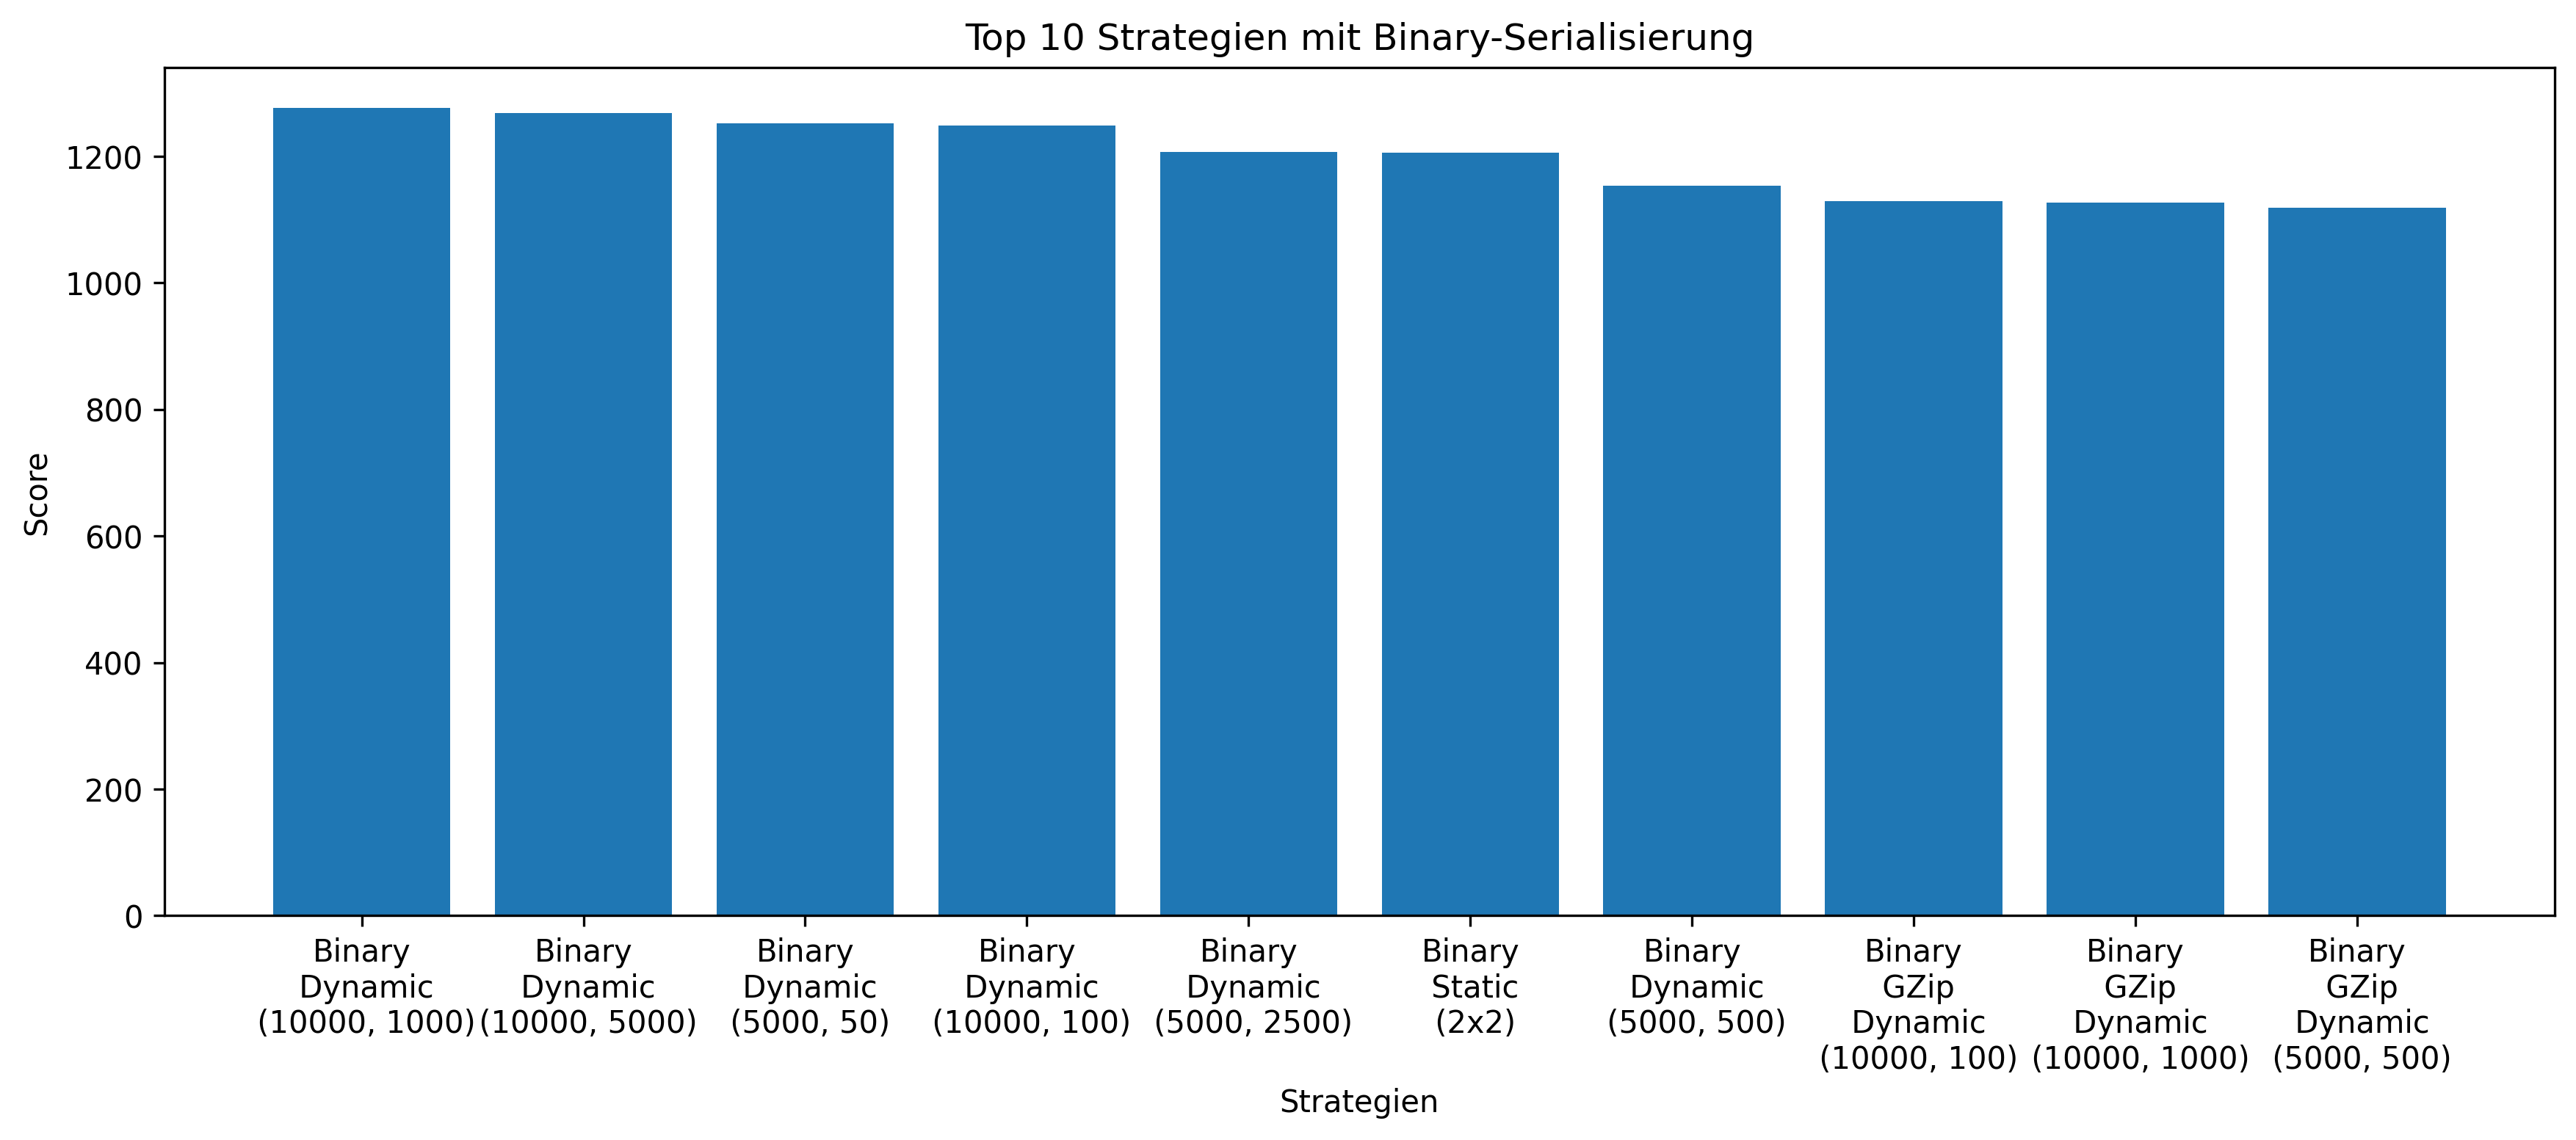
\includegraphics[width=1\textwidth]{images/plots/Binary.png}
    \caption{Beste Binären-Strategien nach dem Score-System aller Kategorien}
    \label{fig:topStratBin}
\end{figure}

\begin{figure}[htp]
    \centering
    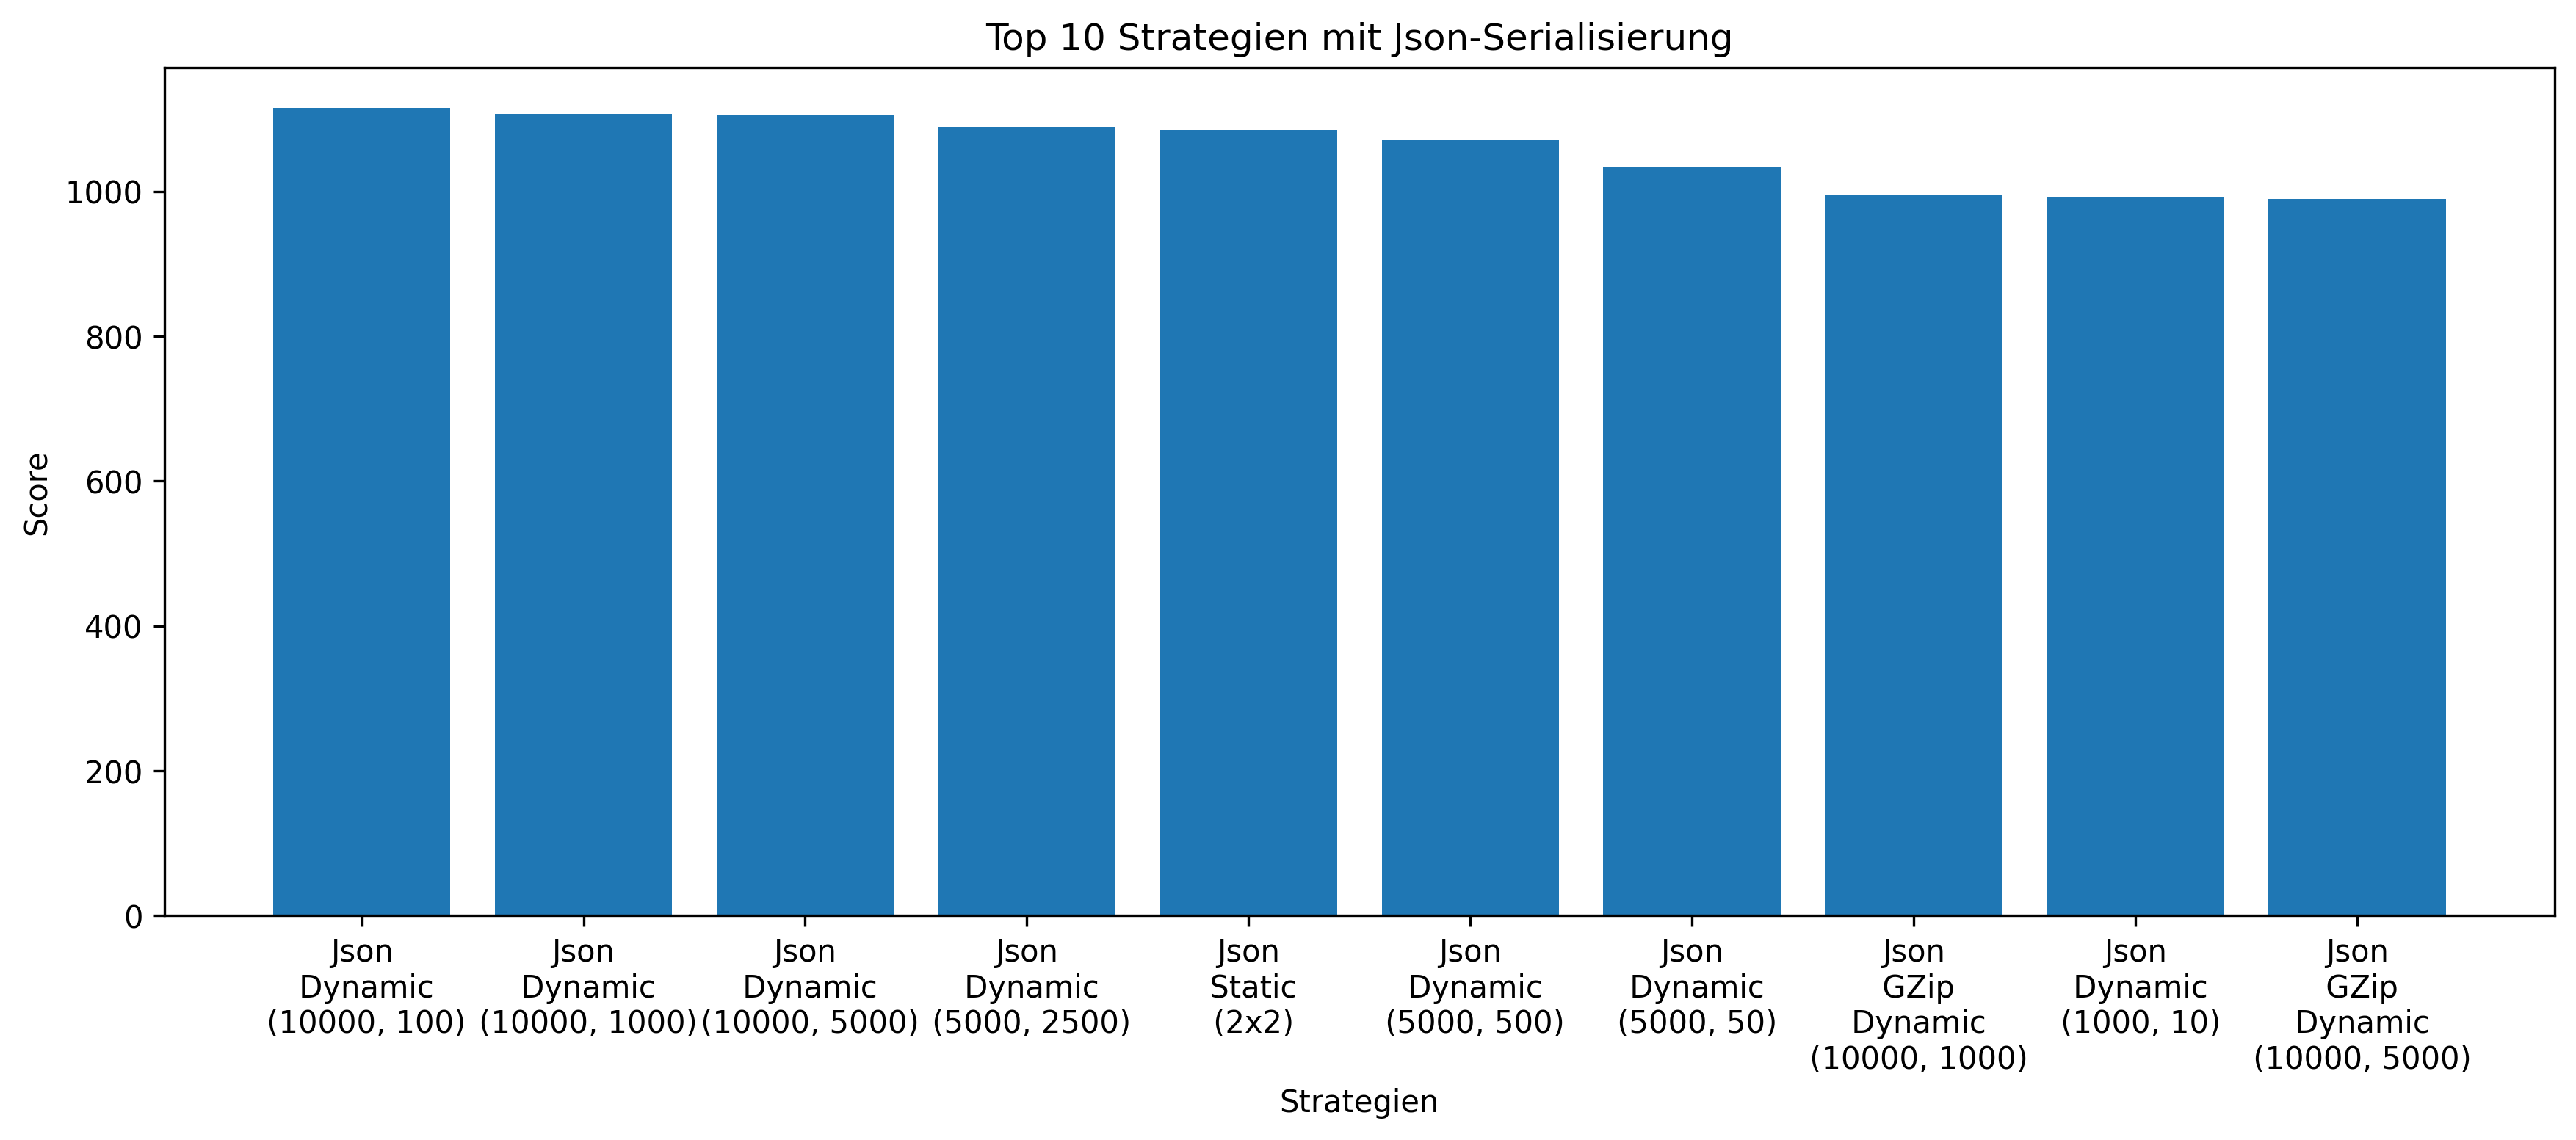
\includegraphics[width=1\textwidth]{images/plots/Json.png}
    \caption{Beste JSON-Strategien nach dem Score-System aller Kategorien}
    \label{fig:topStratJson}
\end{figure}

\begin{figure}[htp]
    \centering
    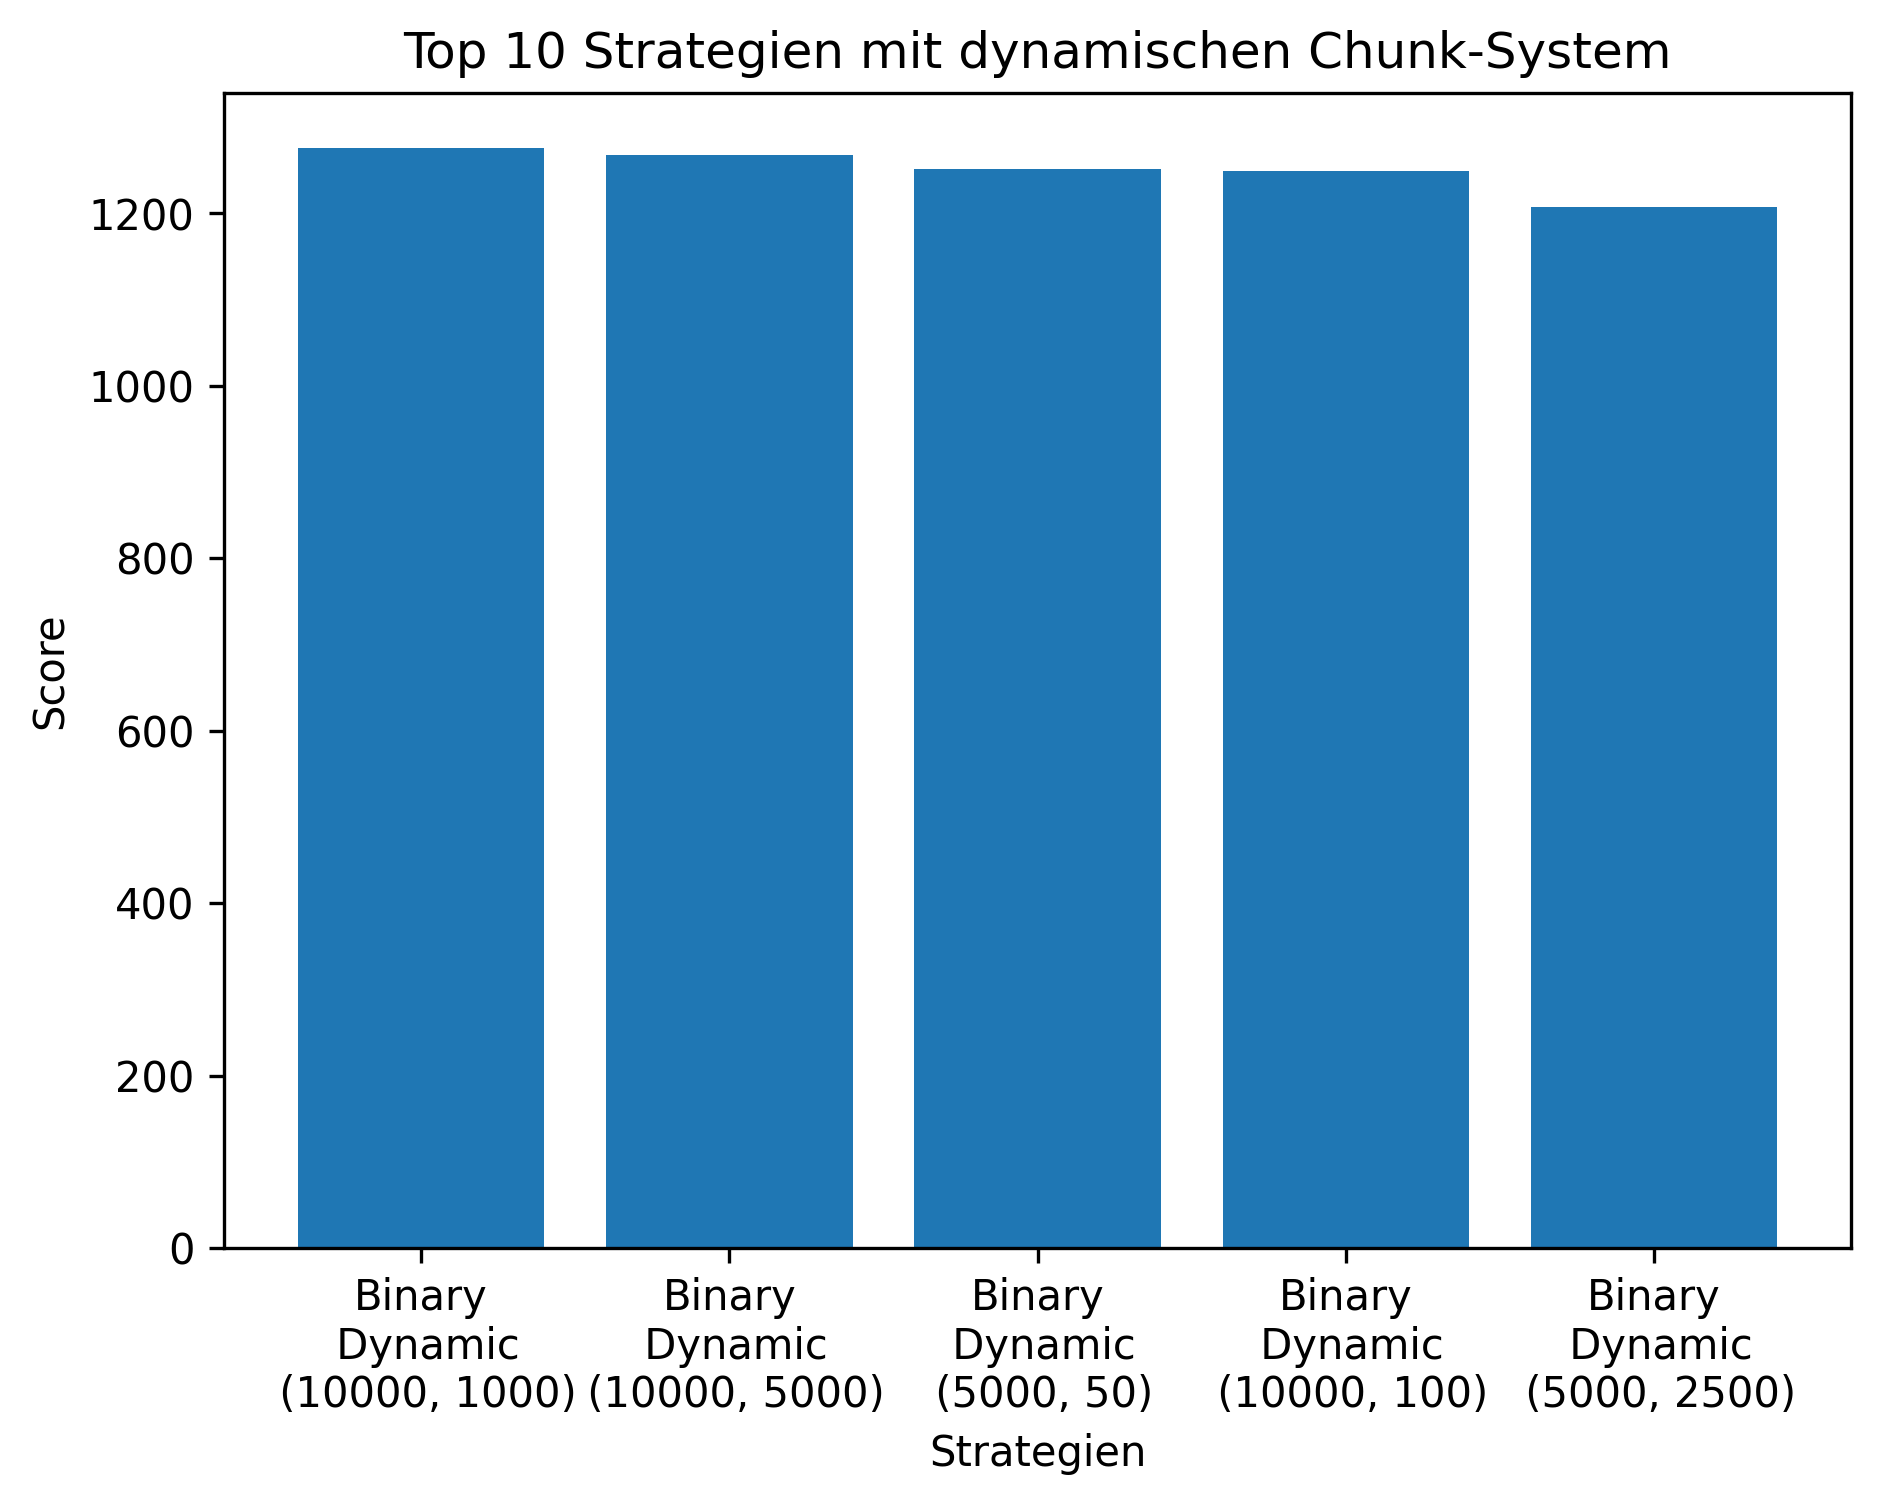
\includegraphics[width=0.7\textwidth]{images/plots/dynamisch.png}
    \caption{Beste Strategien mit dynamischen Chunk-System nach dem Score-System aller Kategorien}
    \label{fig:topDynamic}
\end{figure}

\begin{figure}[htp]
    \centering
    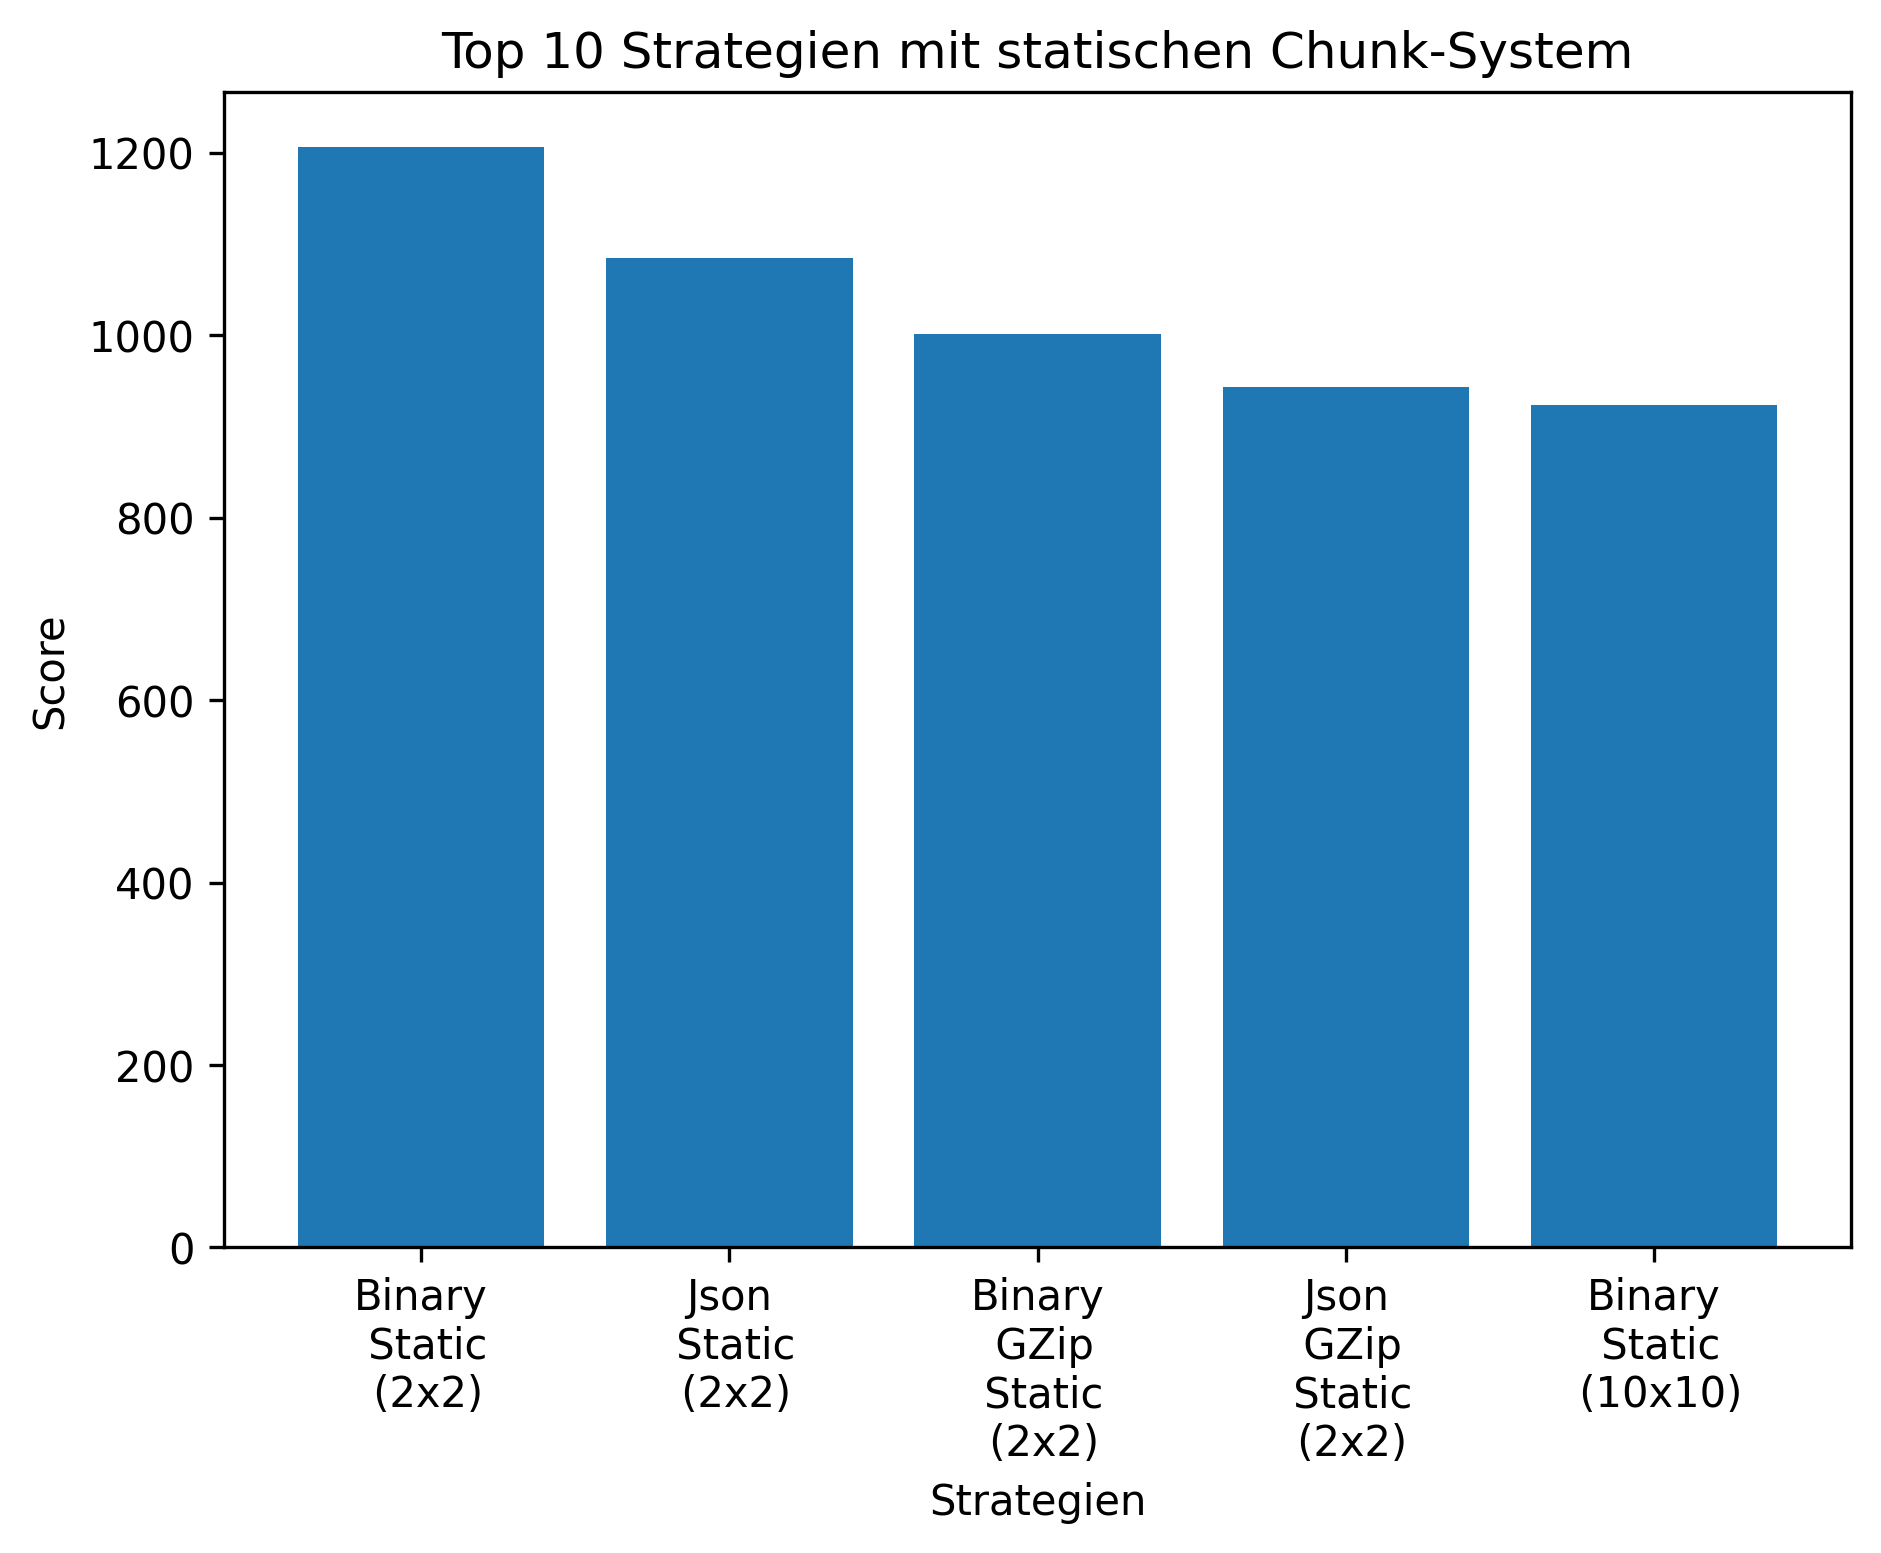
\includegraphics[width=0.7\textwidth]{images/plots/statisch.png}
    \caption{Beste Strategien mit statischen Chunk-System nach dem Score-System aller Kategorien}
    \label{fig:topStatic}
\end{figure}

\begin{figure}[htp]
    \centering
    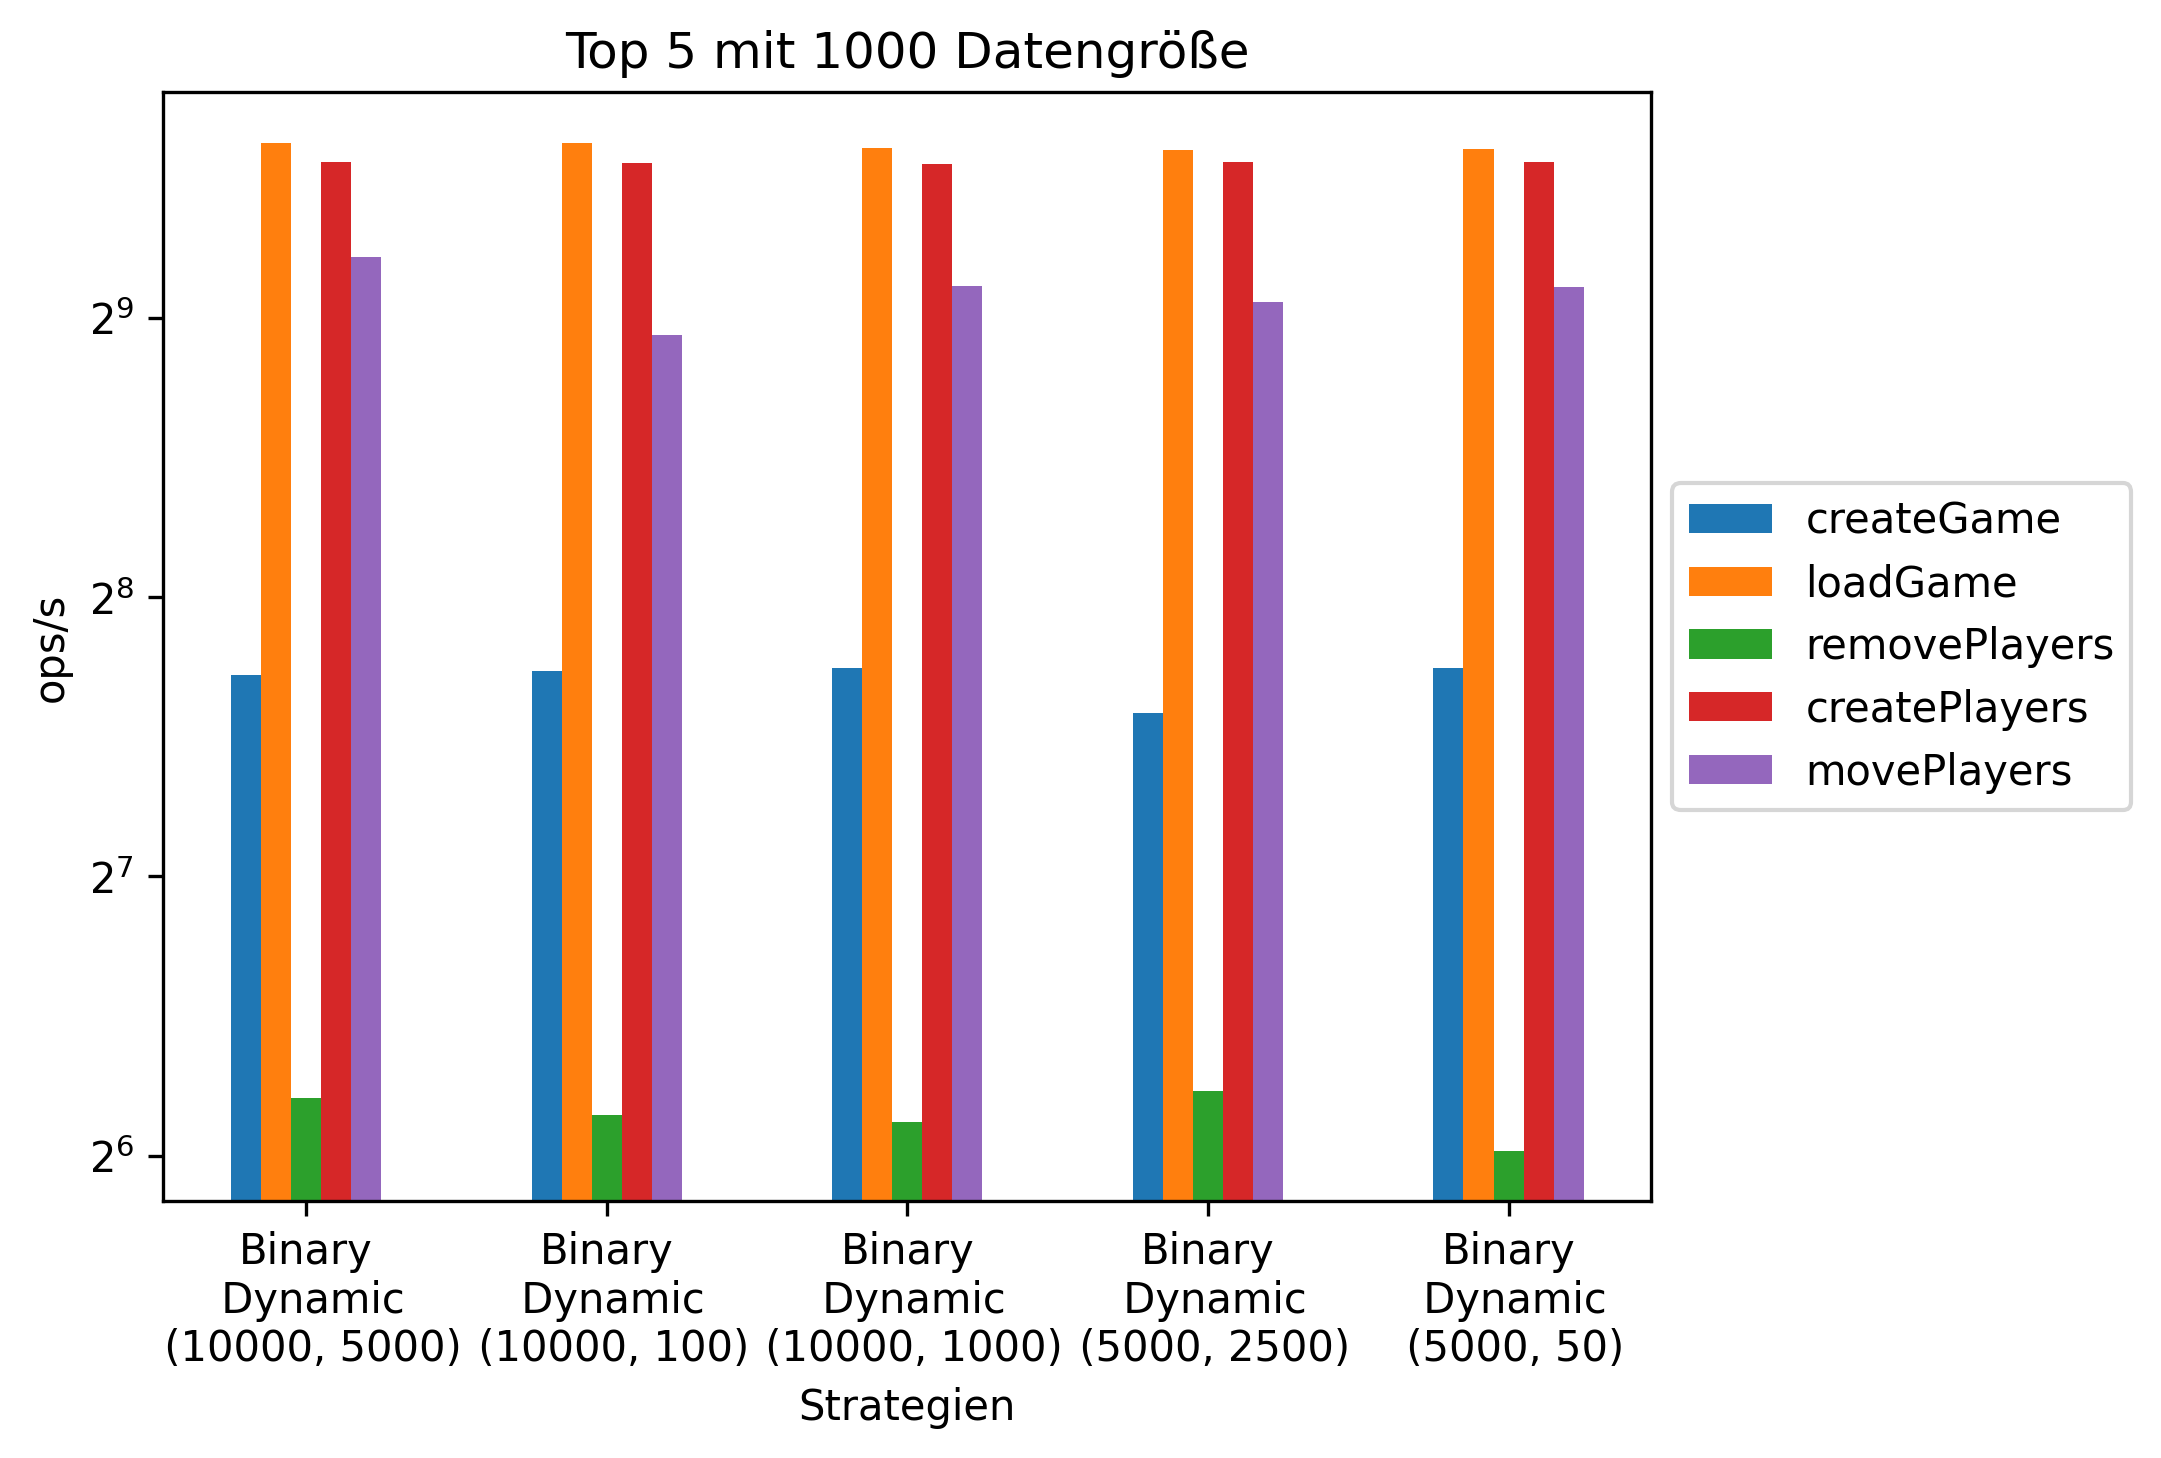
\includegraphics[width=0.7\textwidth]{images/plots/1000.png}
    \caption{Beste Strategien bei einer Datengröße von 1000}
    \label{fig:smallDataCount}
\end{figure}

\begin{figure}[htp]
    \centering
    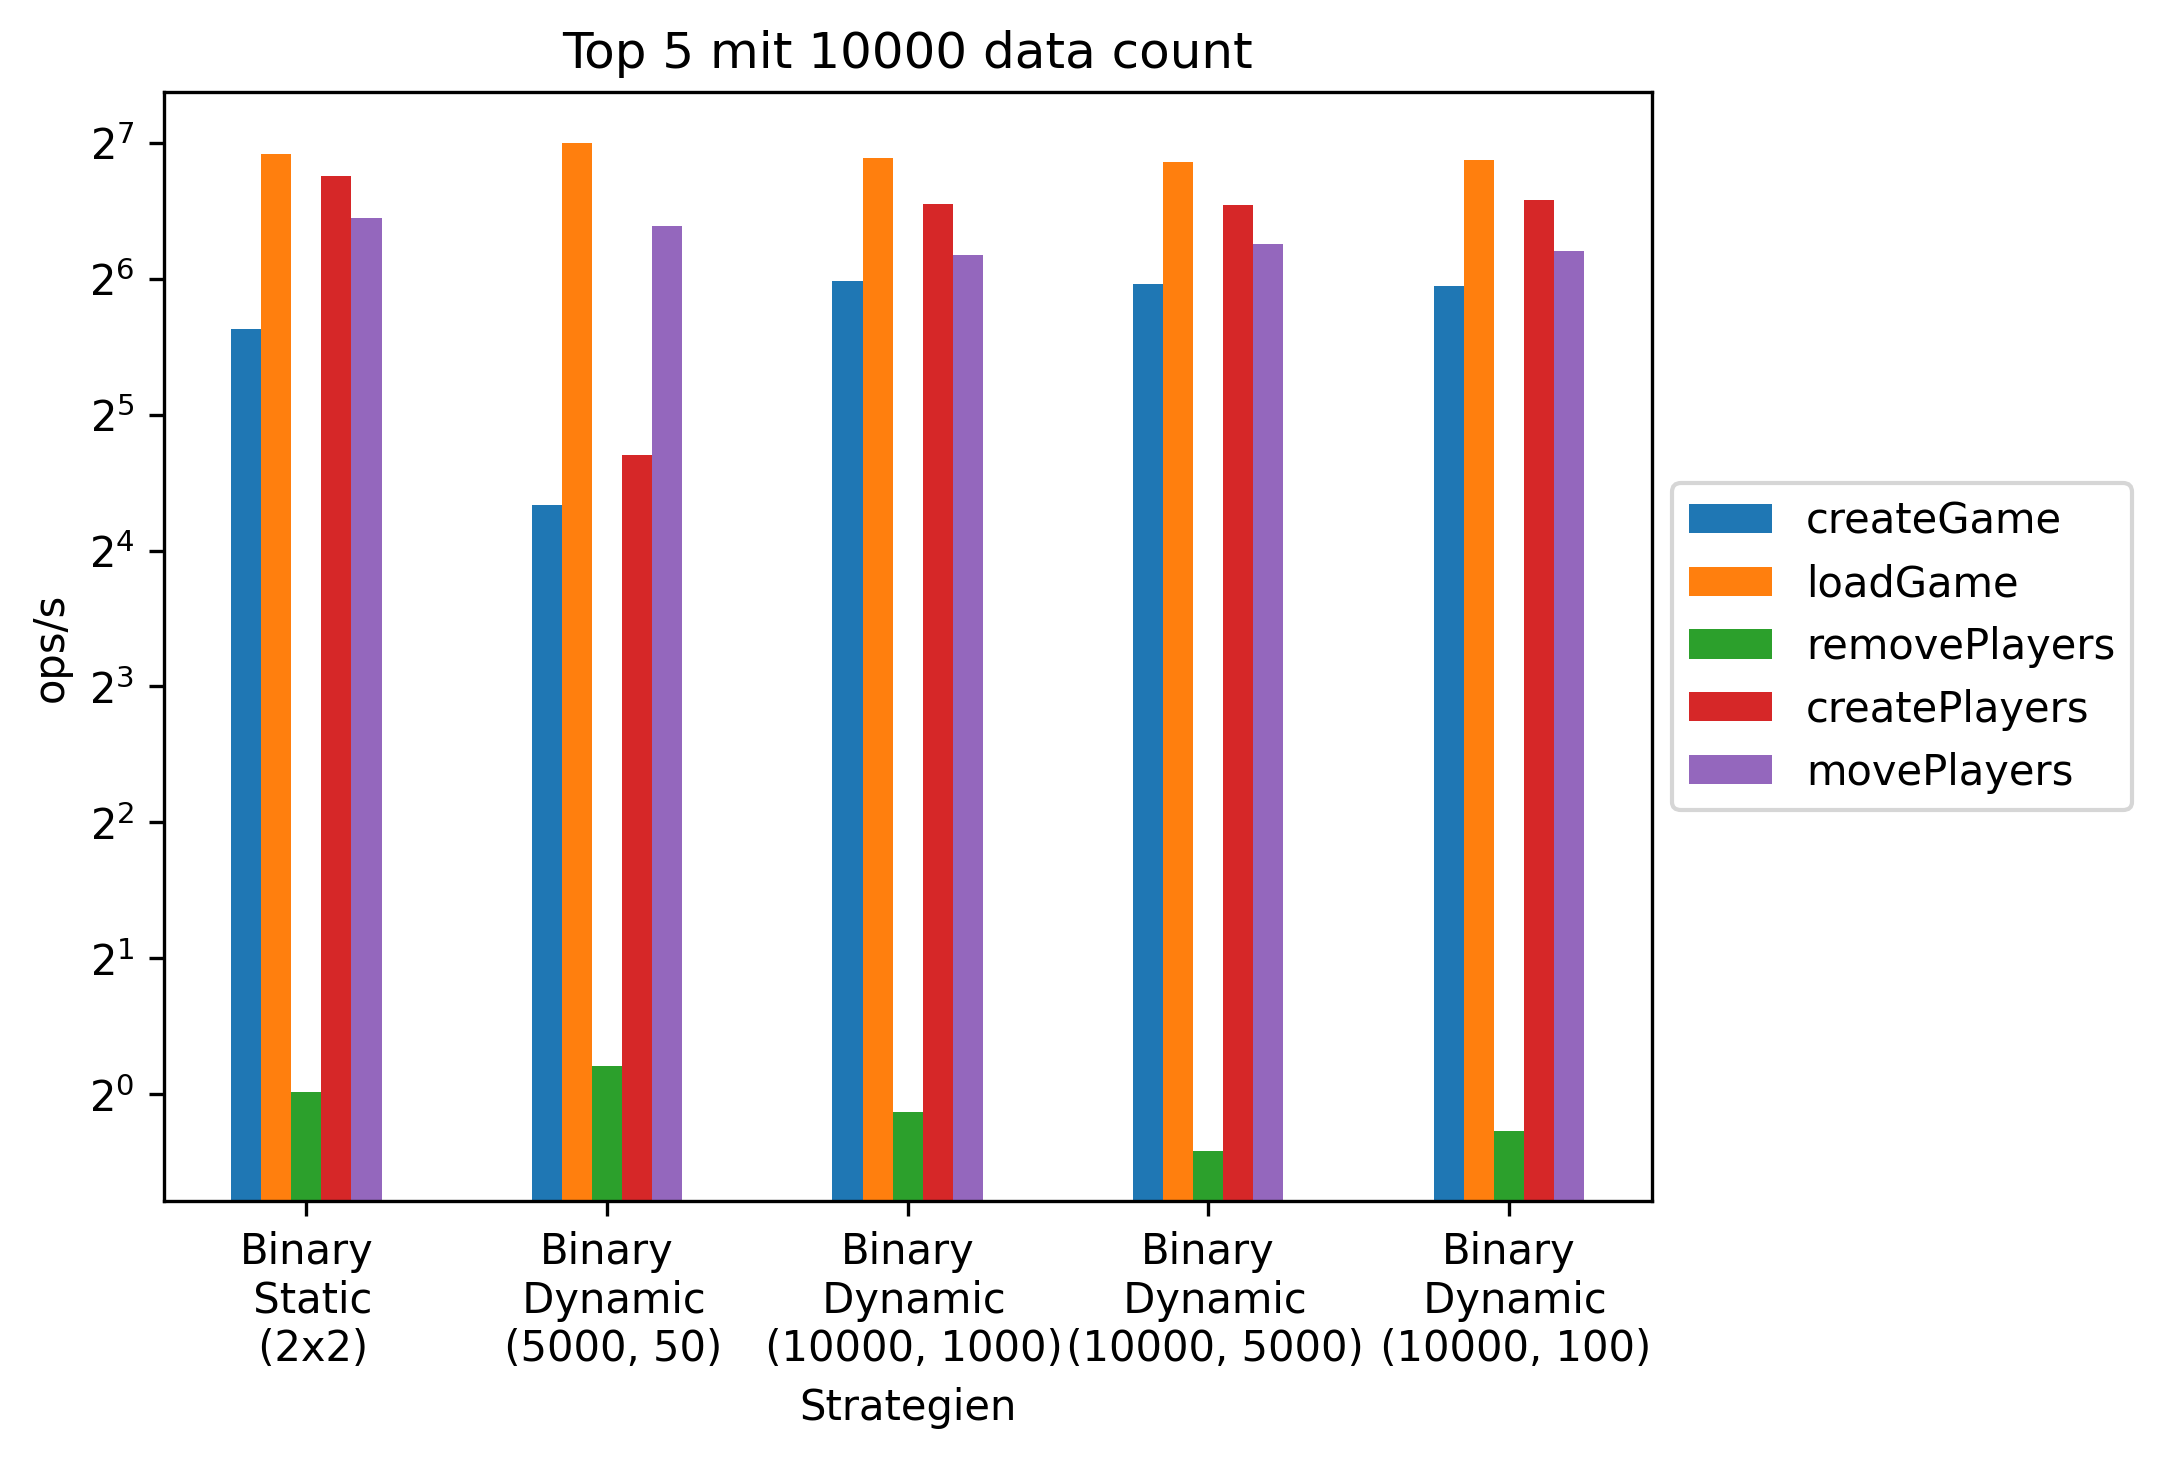
\includegraphics[width=0.7\textwidth]{images/plots/10000.png}
    \caption{Beste Strategien bei einer Datengröße von 10000}
    \label{fig:middleDataCount}
\end{figure}

\begin{figure}[htp]
    \centering
    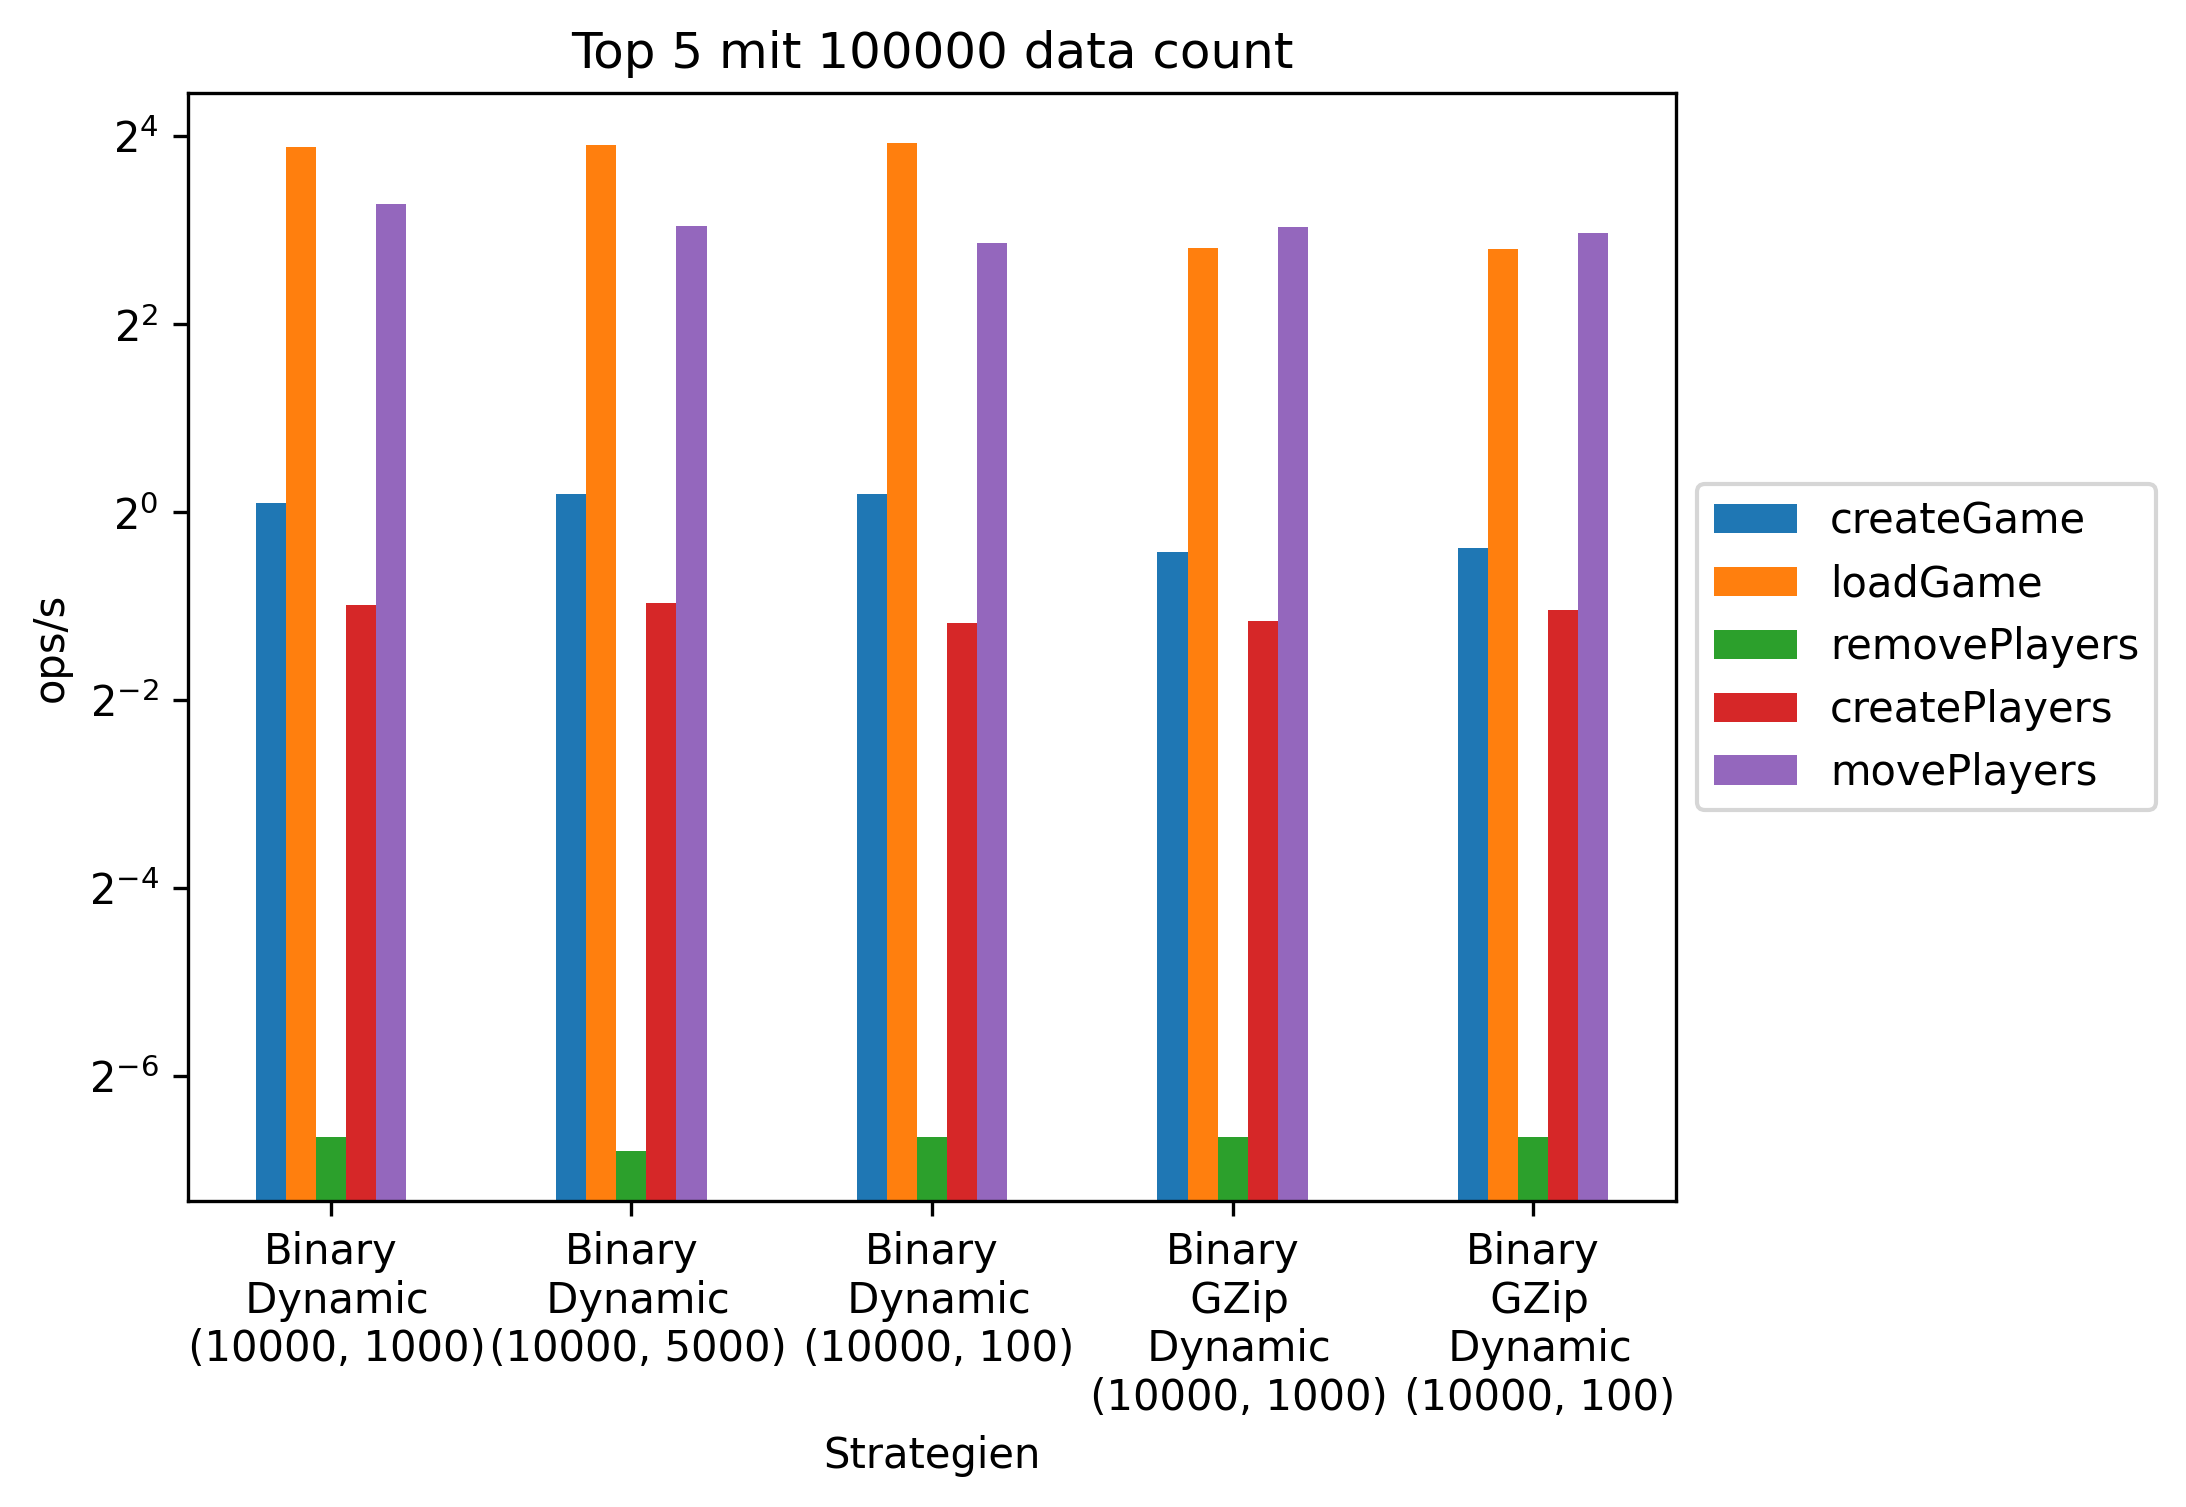
\includegraphics[width=0.7\textwidth]{images/plots/100000.png}
    \caption{Beste Strategien bei einer Daten-Anzahl von 100000}
    \label{fig:bigDataCount}
\end{figure}

\begin{figure}[htp]
    \centering
    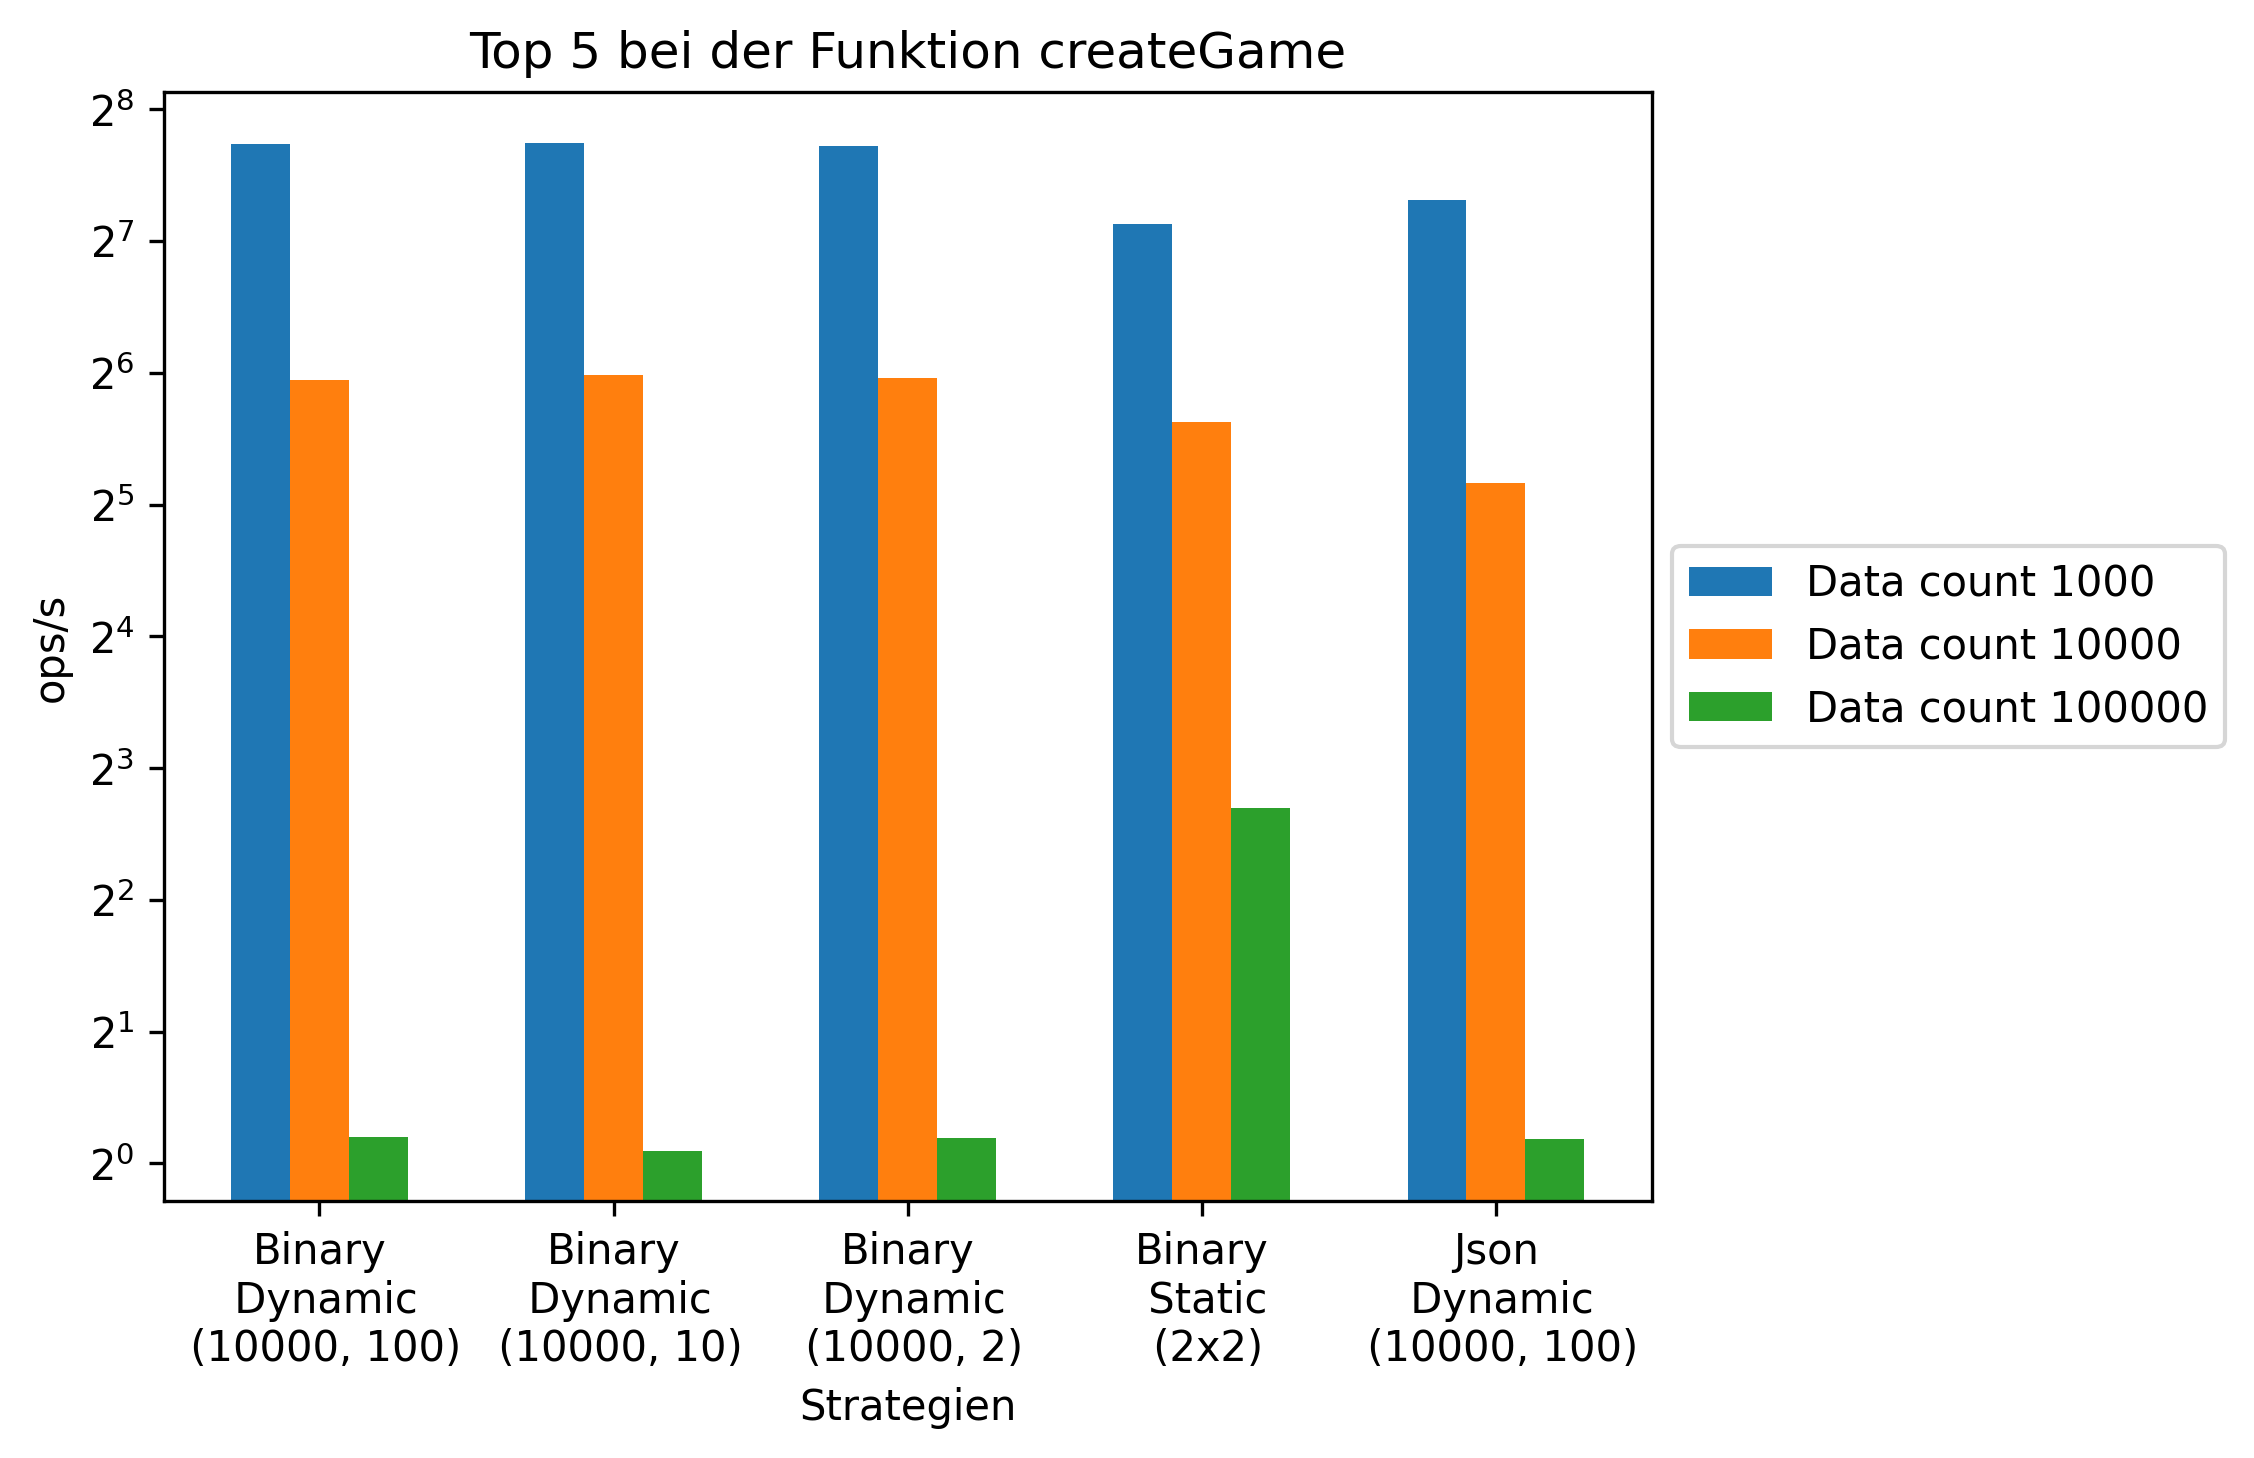
\includegraphics[width=0.7\textwidth]{images/plots/createGame.png}
    \caption{Beste Strategien für die Funktion createGame}
    \label{fig:createGame}
\end{figure}

\begin{figure}[htp]
    \centering
    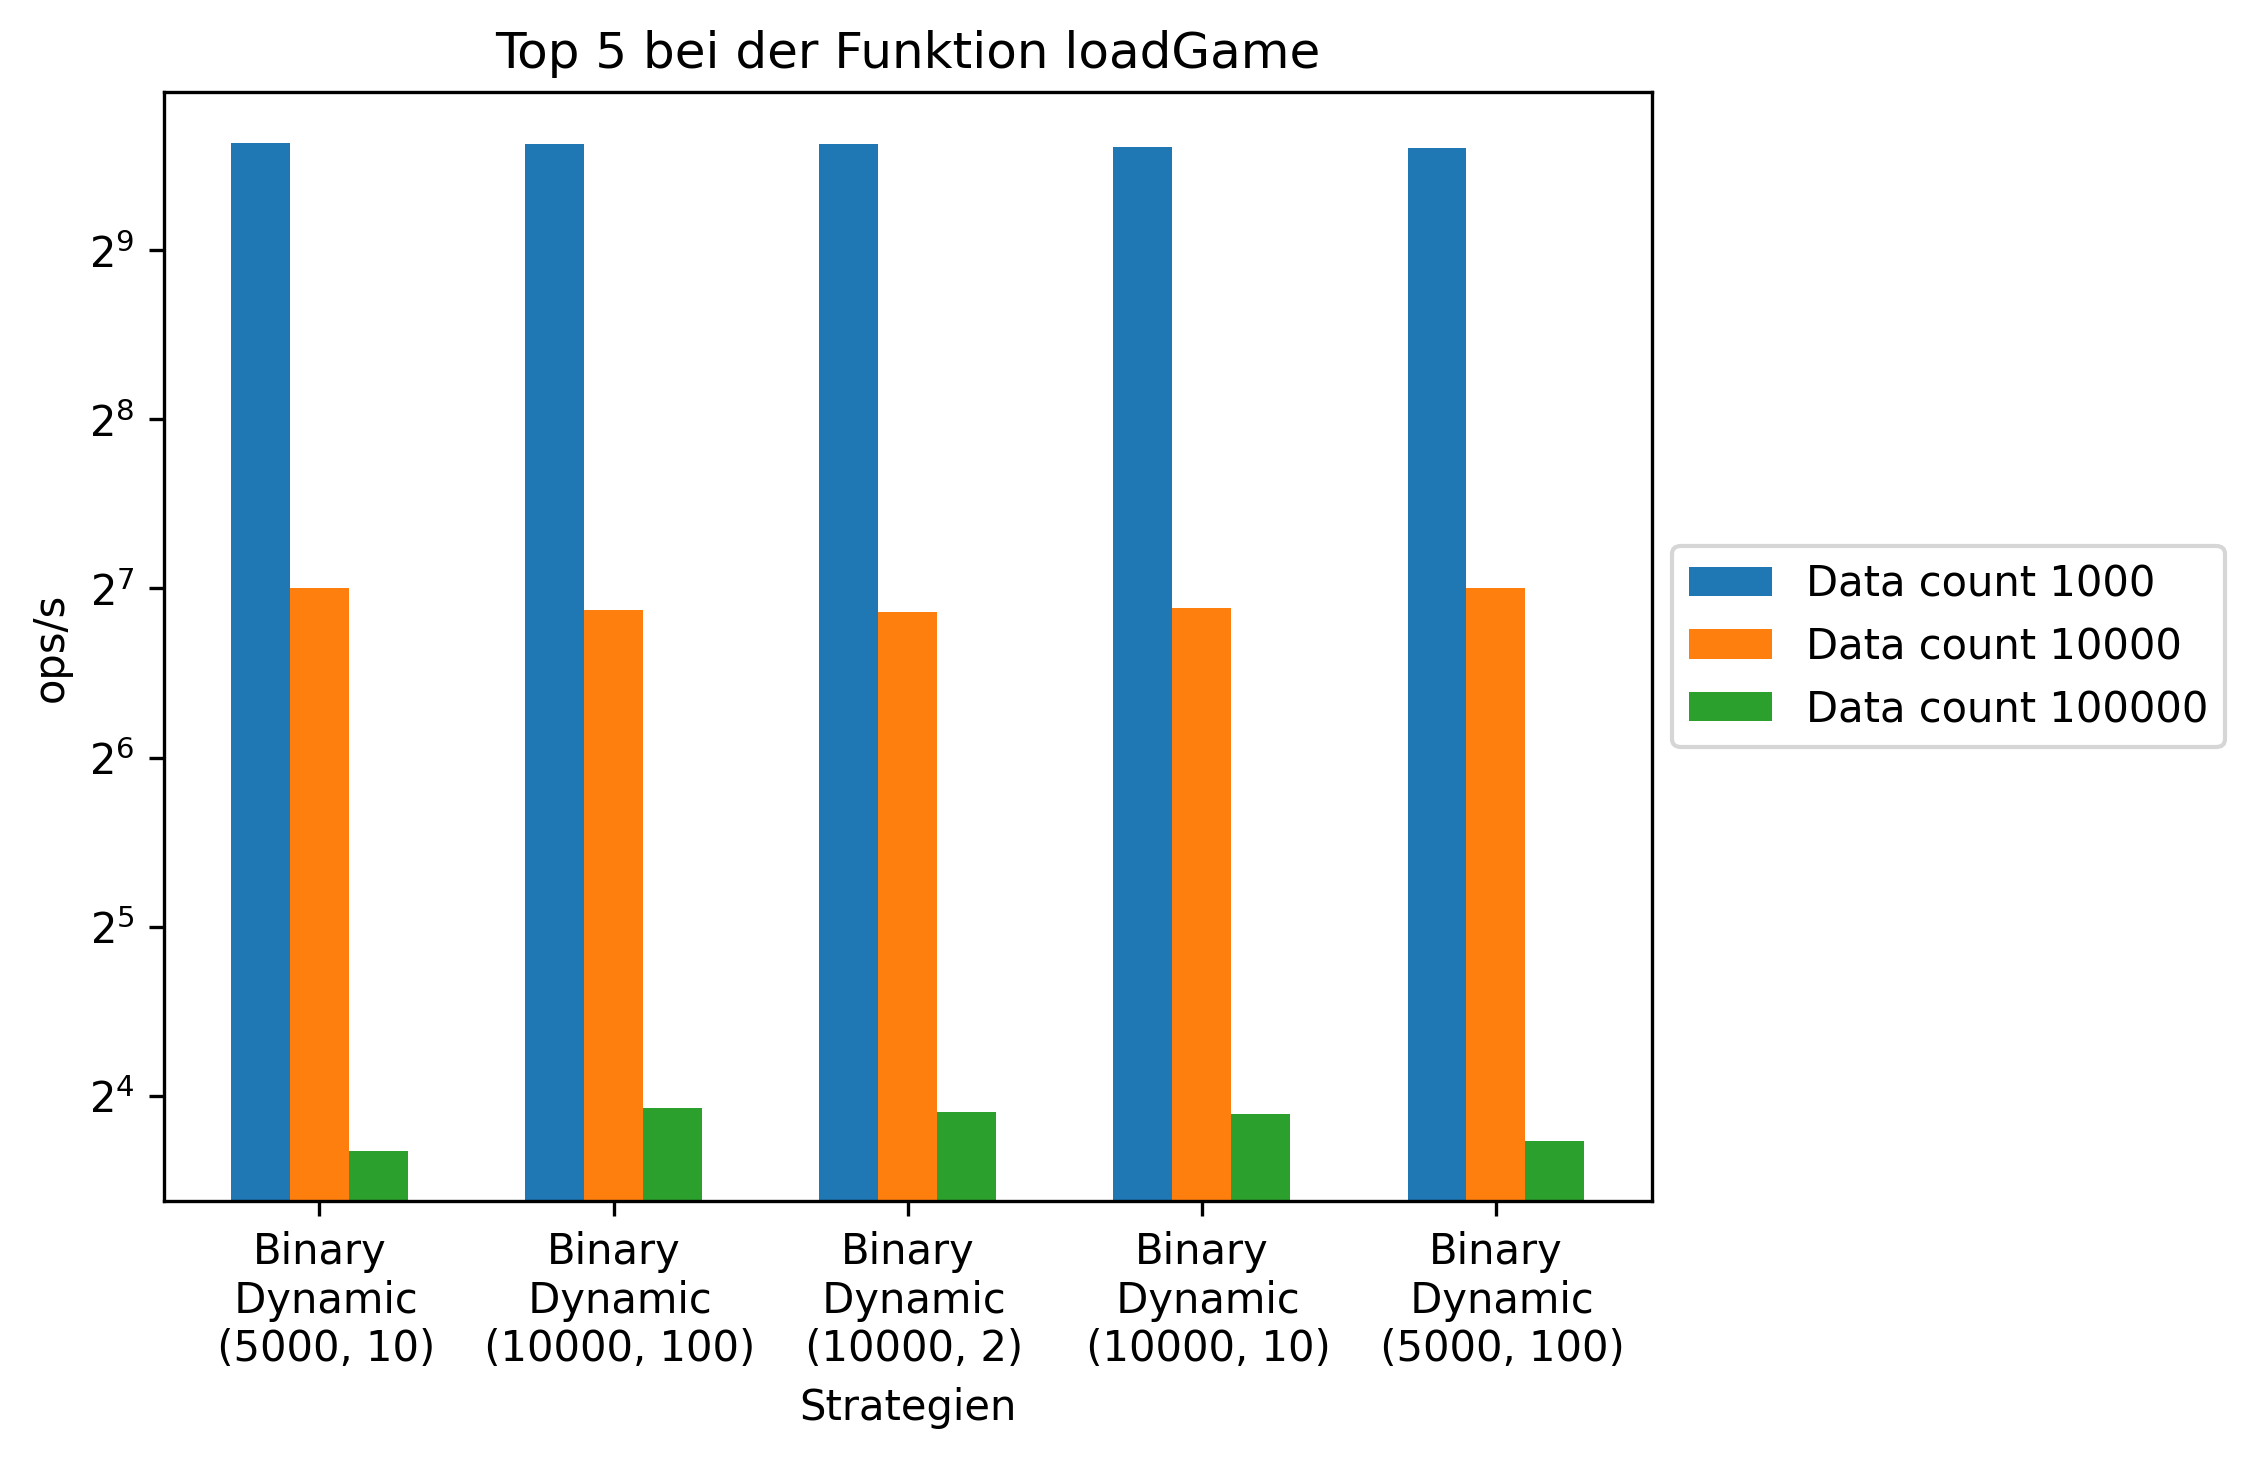
\includegraphics[width=0.7\textwidth]{images/plots/loadGame.png}
    \caption{Beste Strategien für die Funktion loadGame}
    \label{fig:loadGame}
\end{figure}

\begin{figure}[htp]
    \centering
    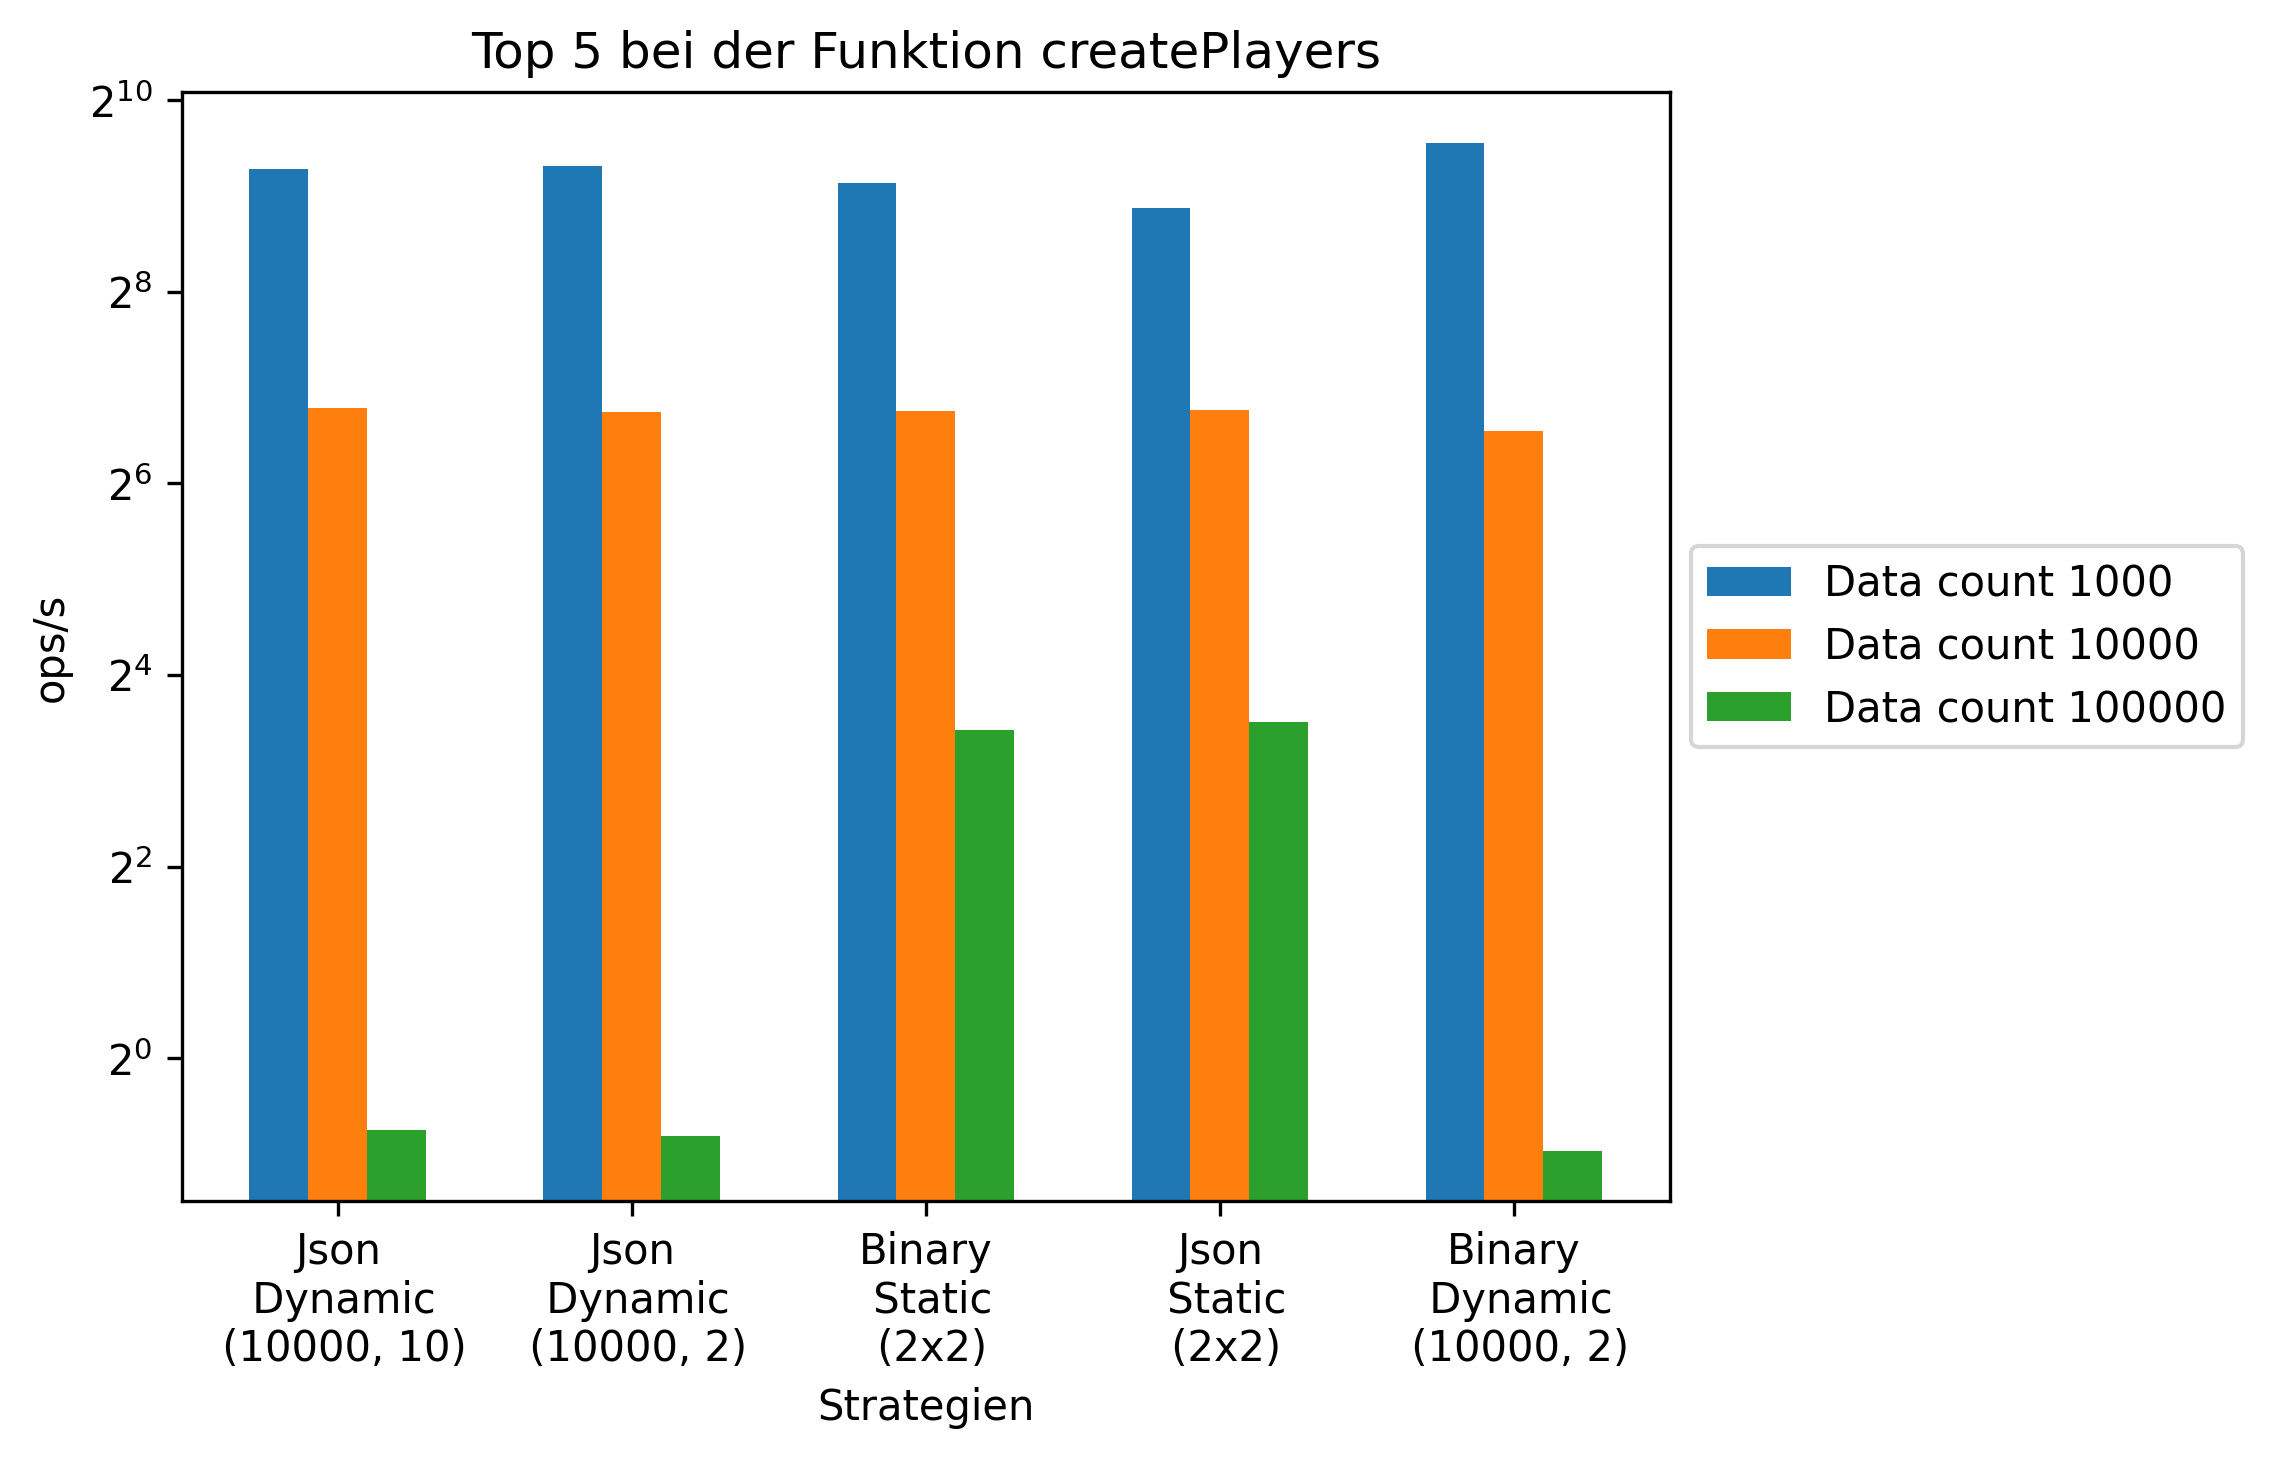
\includegraphics[width=0.7\textwidth]{images/plots/createPlayers.png}
    \caption{Beste Strategien für die Funktion createPlayers}
    \label{fig:createPlayers}
\end{figure}

\begin{figure}[htp]
    \centering
    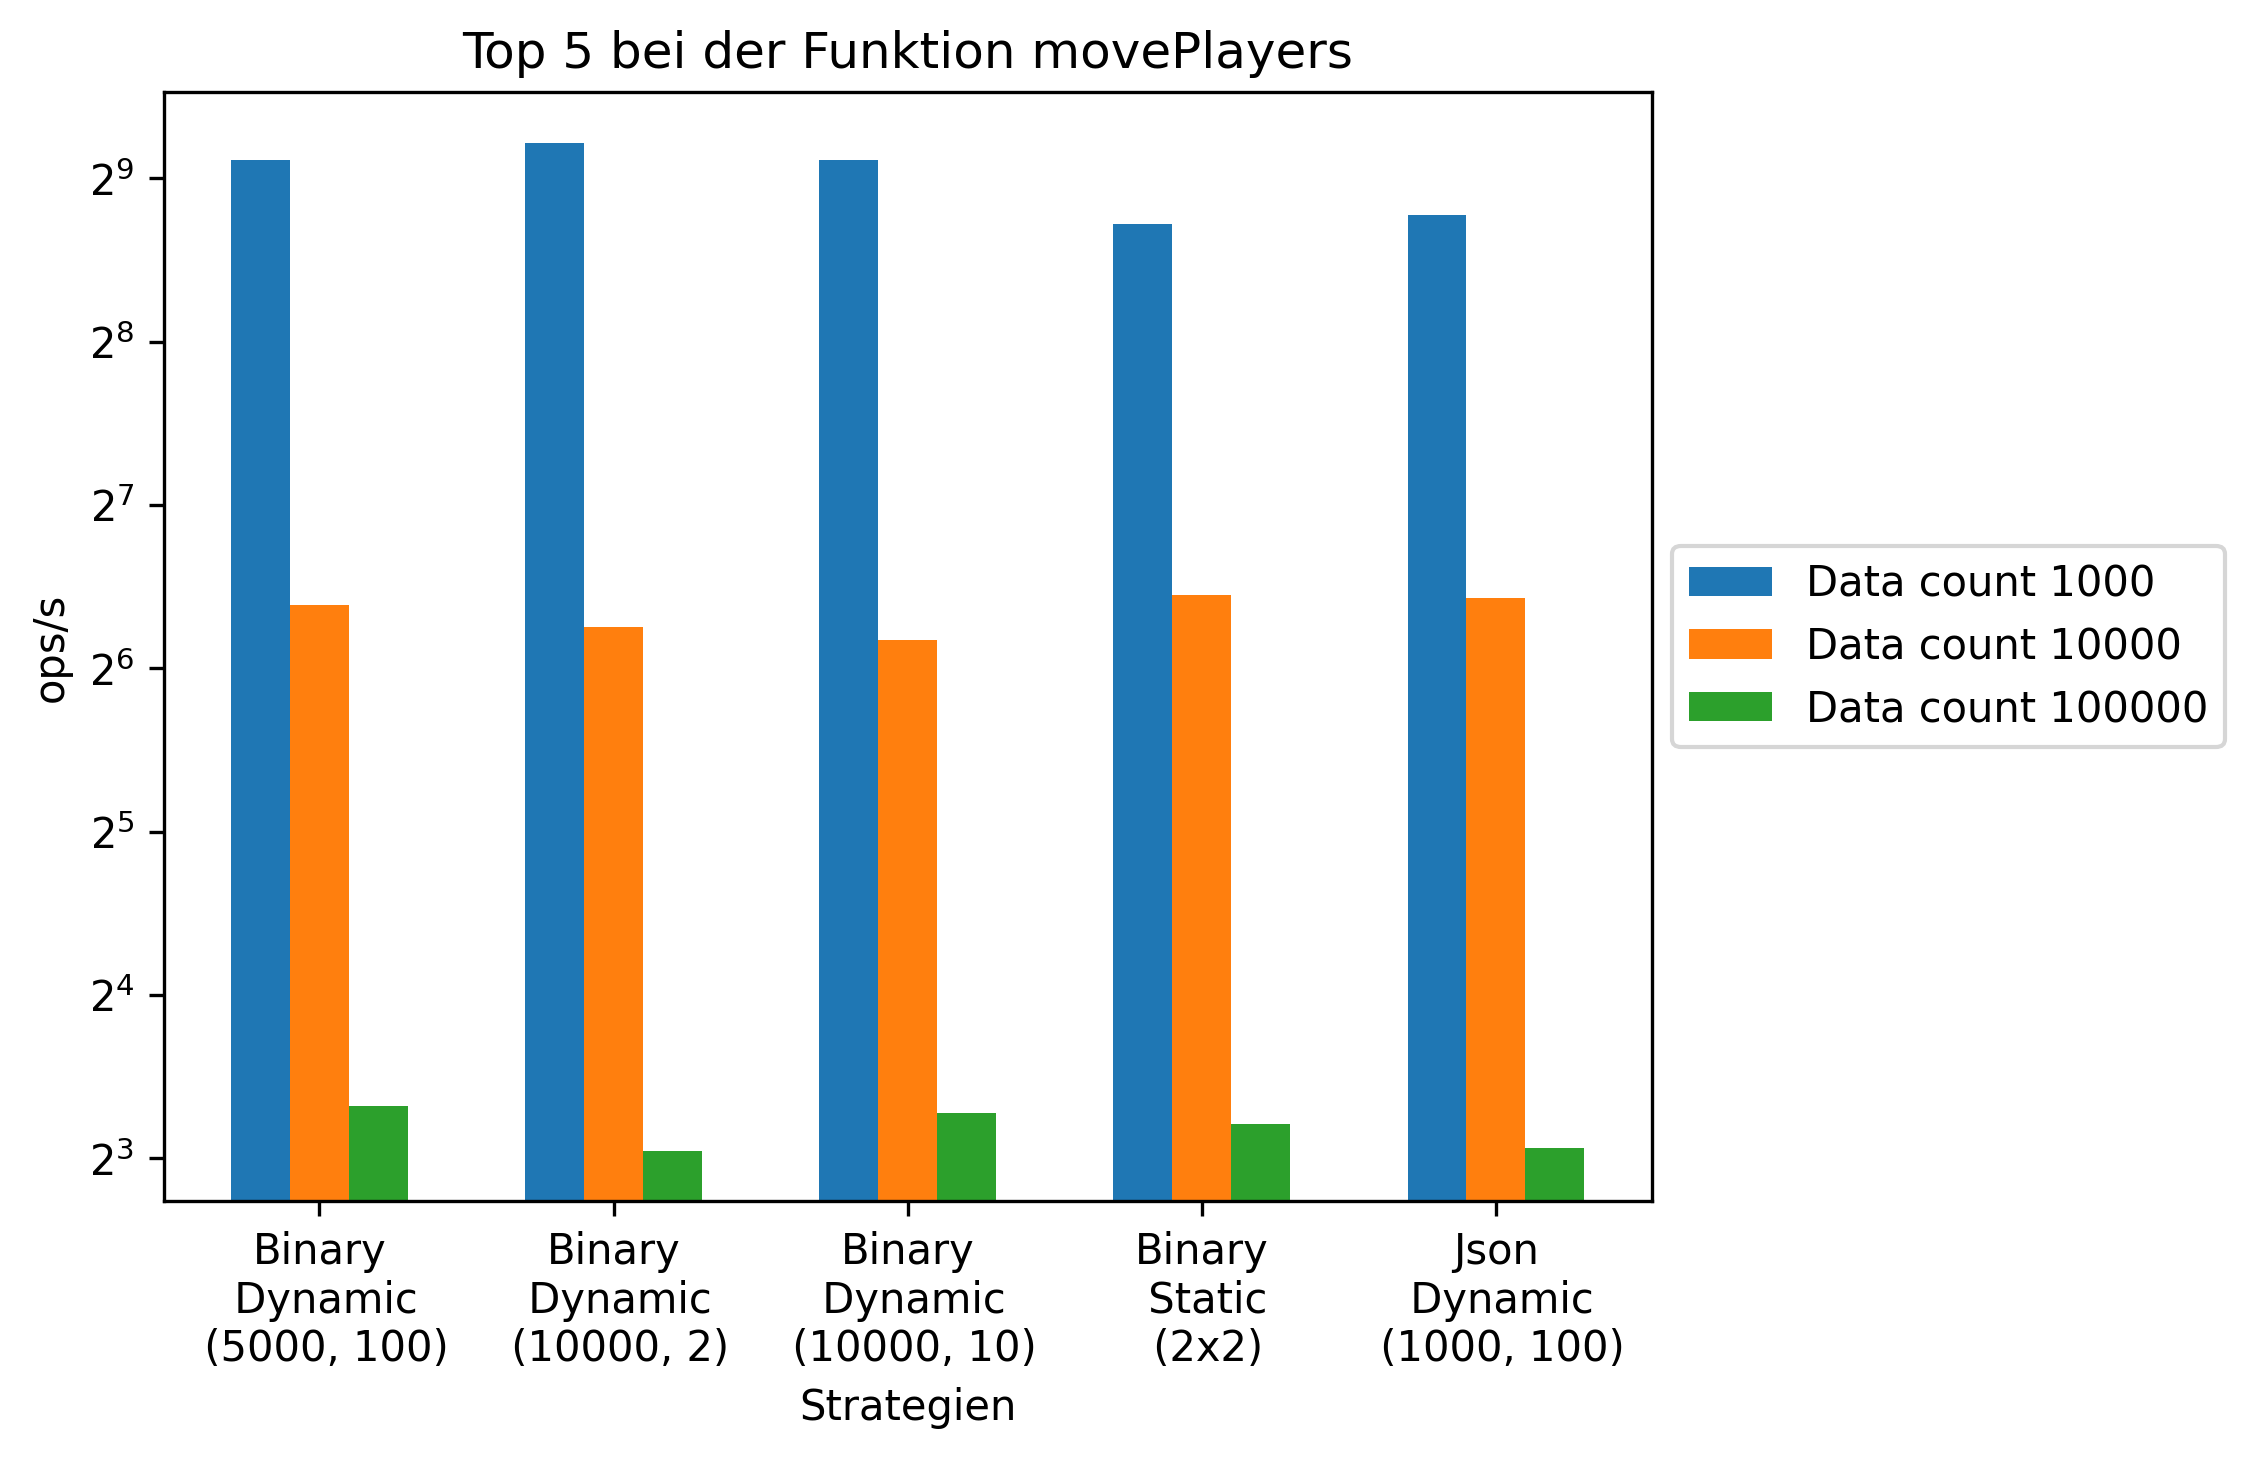
\includegraphics[width=0.7\textwidth]{images/plots/movePlayers.png}
    \caption{Beste Strategien für die Funktion movePlayers}
    \label{fig:movePlayers}
\end{figure}

\begin{figure}[htp]
    \centering
    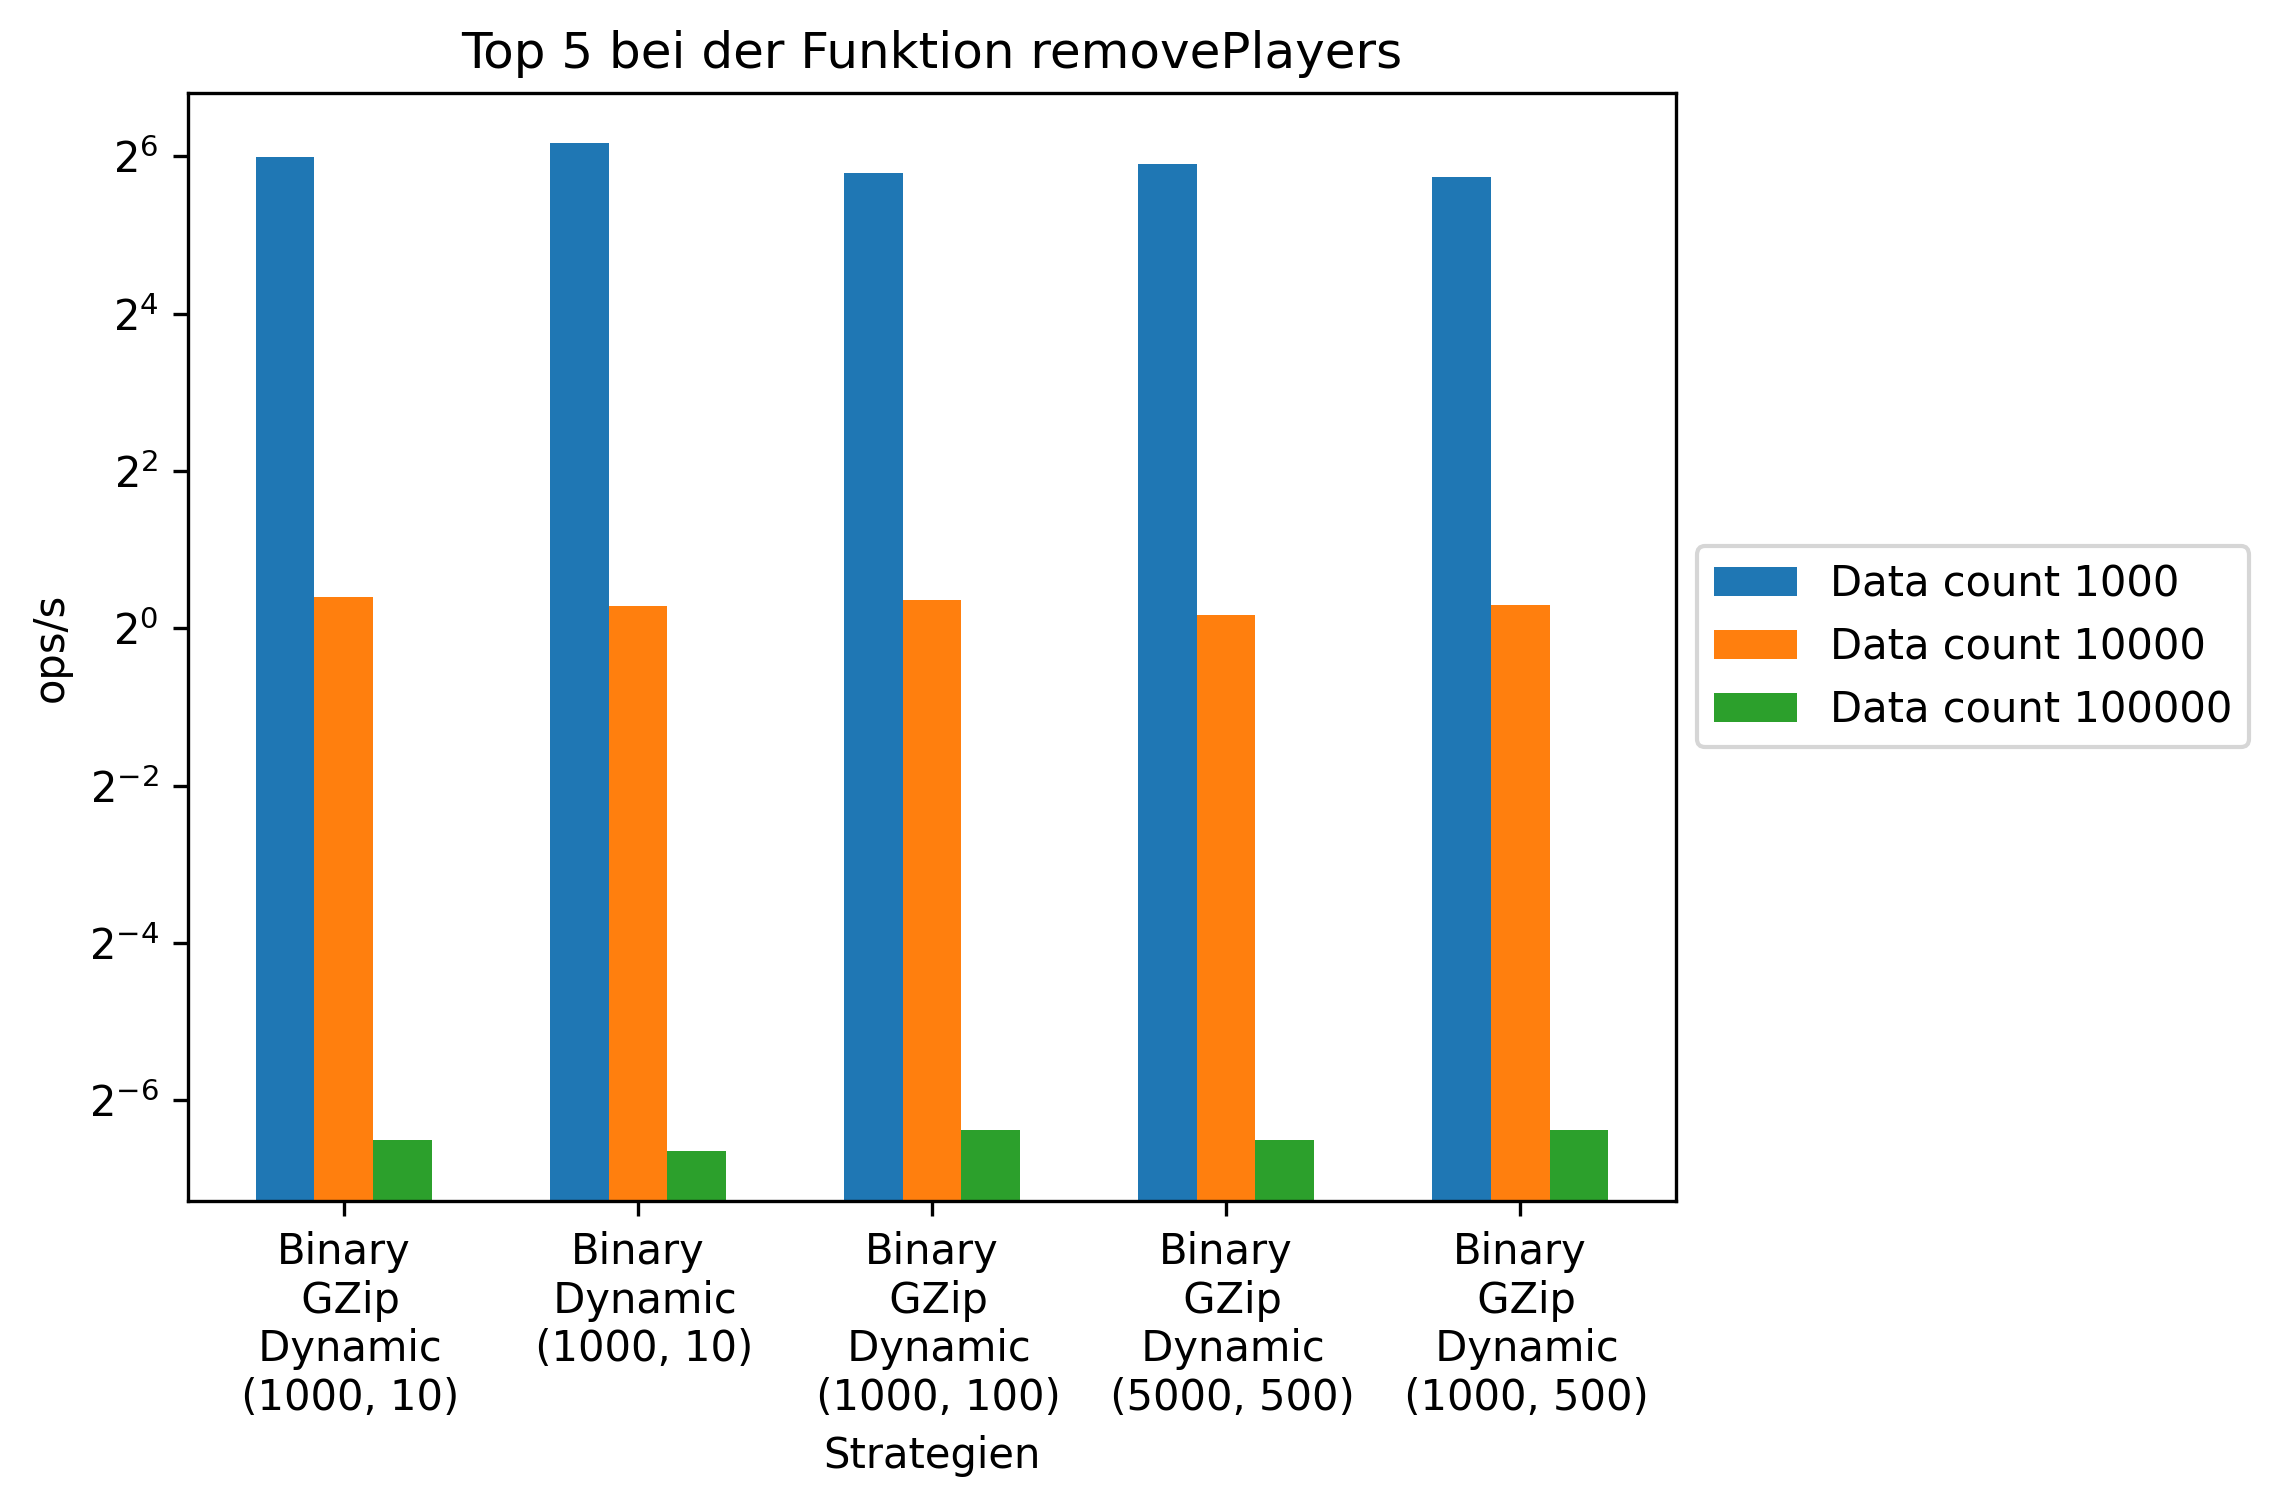
\includegraphics[width=0.7\textwidth]{images/plots/removePlayers.png}
    \caption{Beste Strategien für die Funktion removePlayers}
    \label{fig:removePlayers}
\end{figure}

\begin{figure}[htp]
    \centering
    
\includegraphics[width=1\textwidth]{images/Minecraft_Email.png}
    \caption{Email von Minecraft zu dem Speicher- und Ladesystem}
    \label{fig:minecraftMail}
\end{figure}

\begin{figure}[htp]
    \centering
    
\includegraphics[width=1\textwidth]{images/Factorio_Email.png}
    \caption{Email von Factorio zu dem Speicher- und Ladesystem}
    \label{fig:factorioMail}
\end{figure}

\end{document}
